\documentclass[a4wide]{report}

\usepackage{amsmath}
\usepackage[a4paper, total={7in, 10.2in}]{geometry}
\usepackage{graphicx}
\usepackage[portuguese]{babel}
\usepackage[utf8]{inputenc}


\begin{document}

\noindent
{\bf Rafael V. Cacilhas  - Relatório 08 (\today)}

\vspace{0.5cm}

\section*{Exercício 1}

\subsection*{a) }
Na Figura \ref{dinamica} estão os resultados da posição e velocidade para os três métodos. Nesta escala não há diferenças visíveis entre os três métodos, de modo que foi feito um gráfico do erro absoluto da posição para os três métodos, que pode ser visto na Figura \ref{4}.

\begin{figure}[!htb]
\centering
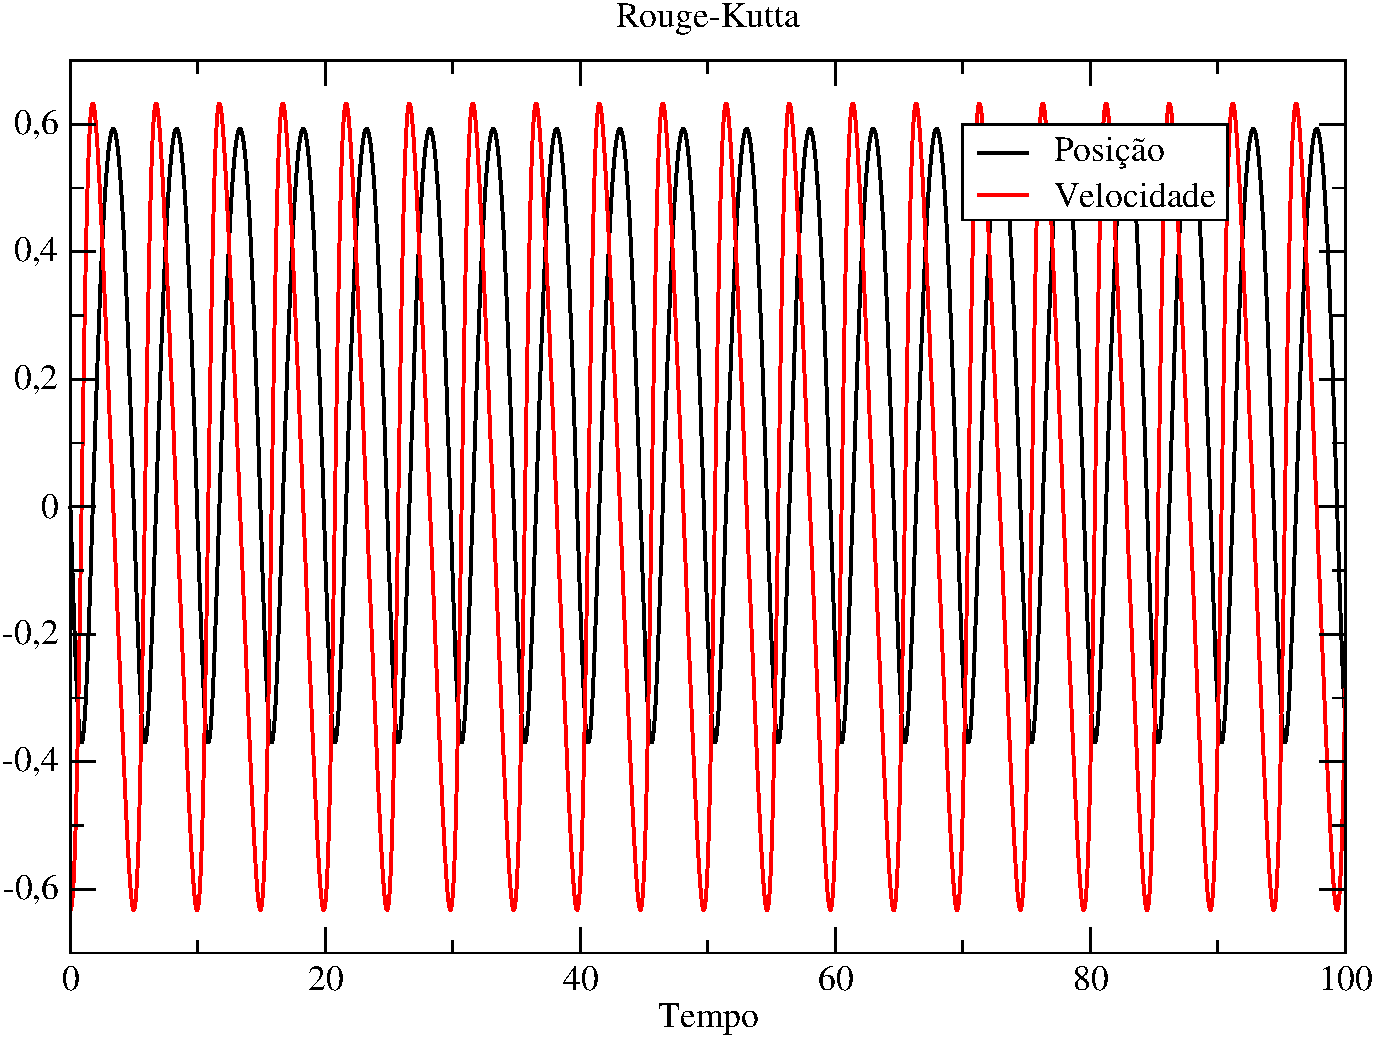
\includegraphics[width=0.32\textwidth]{xevrk.pdf}
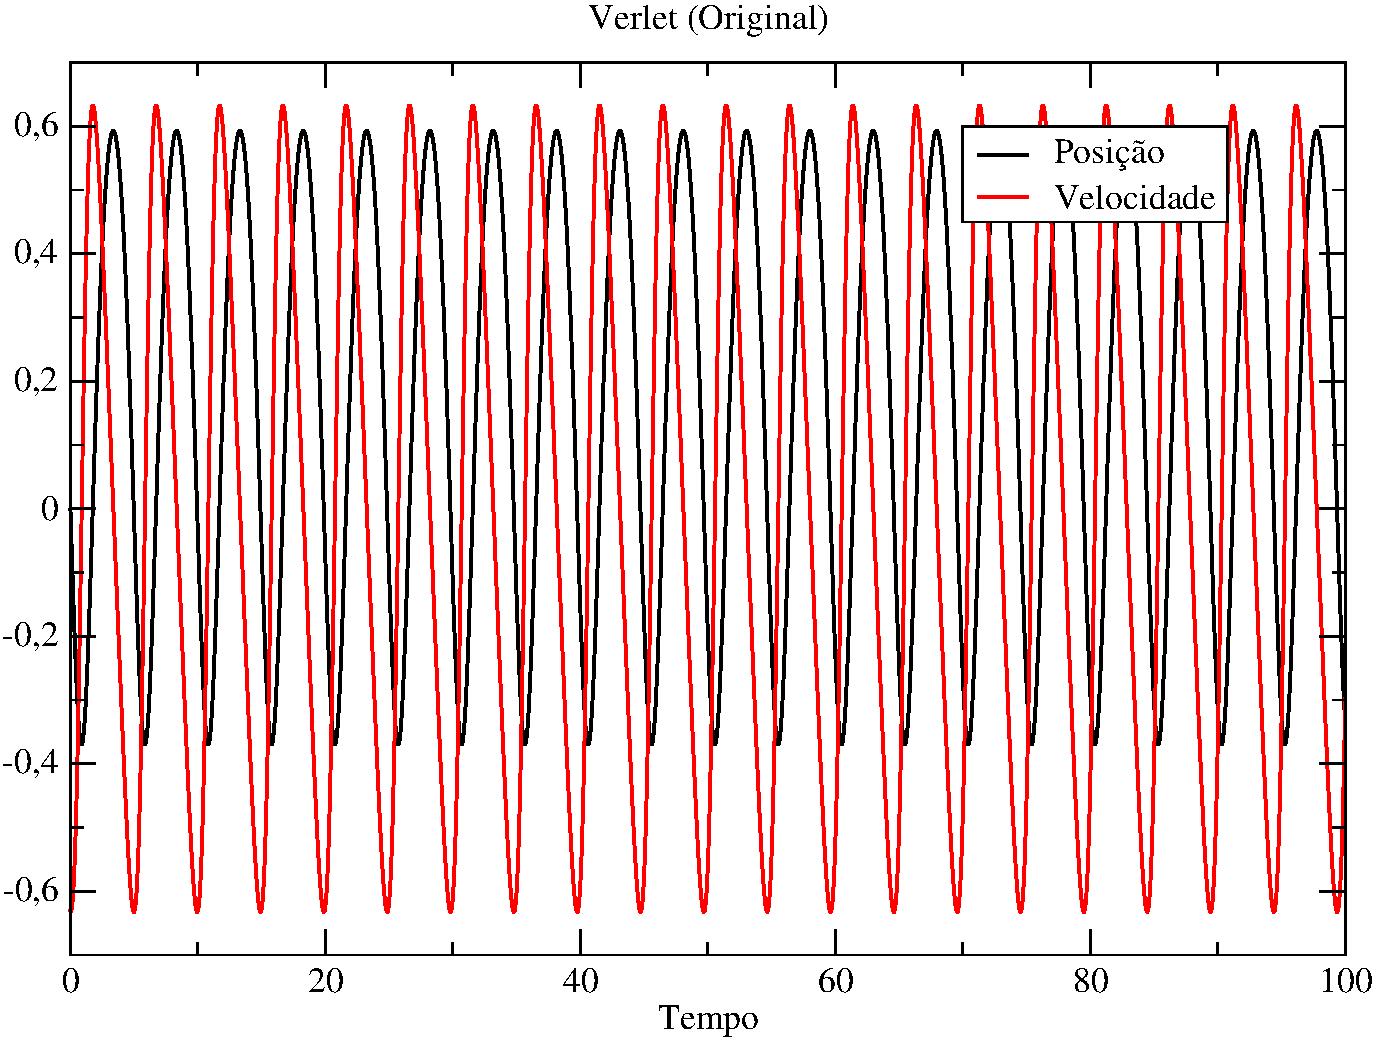
\includegraphics[width=0.32\textwidth]{xevvO.pdf}
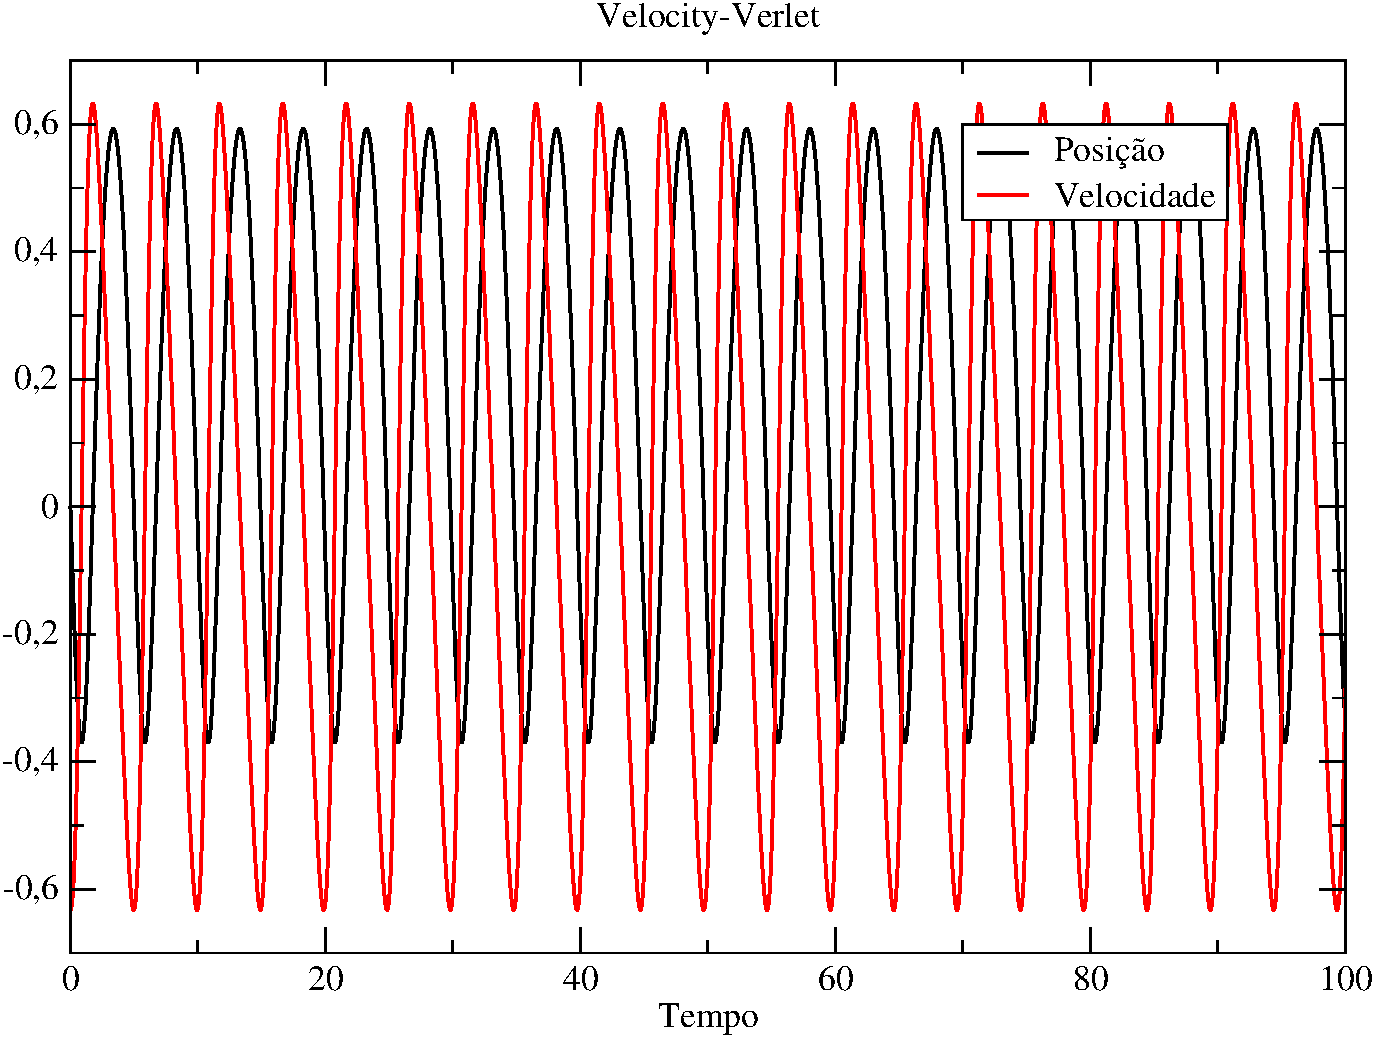
\includegraphics[width=0.32\textwidth]{xevVerletV.pdf}
\caption{Dinâmica resolvida através do método de Rouge-Kutta, Verlet(original) e Velocity-Verlet, respectivamente.}
\label{dinamica}
\end{figure}



\begin{figure}[!htb]
\centering
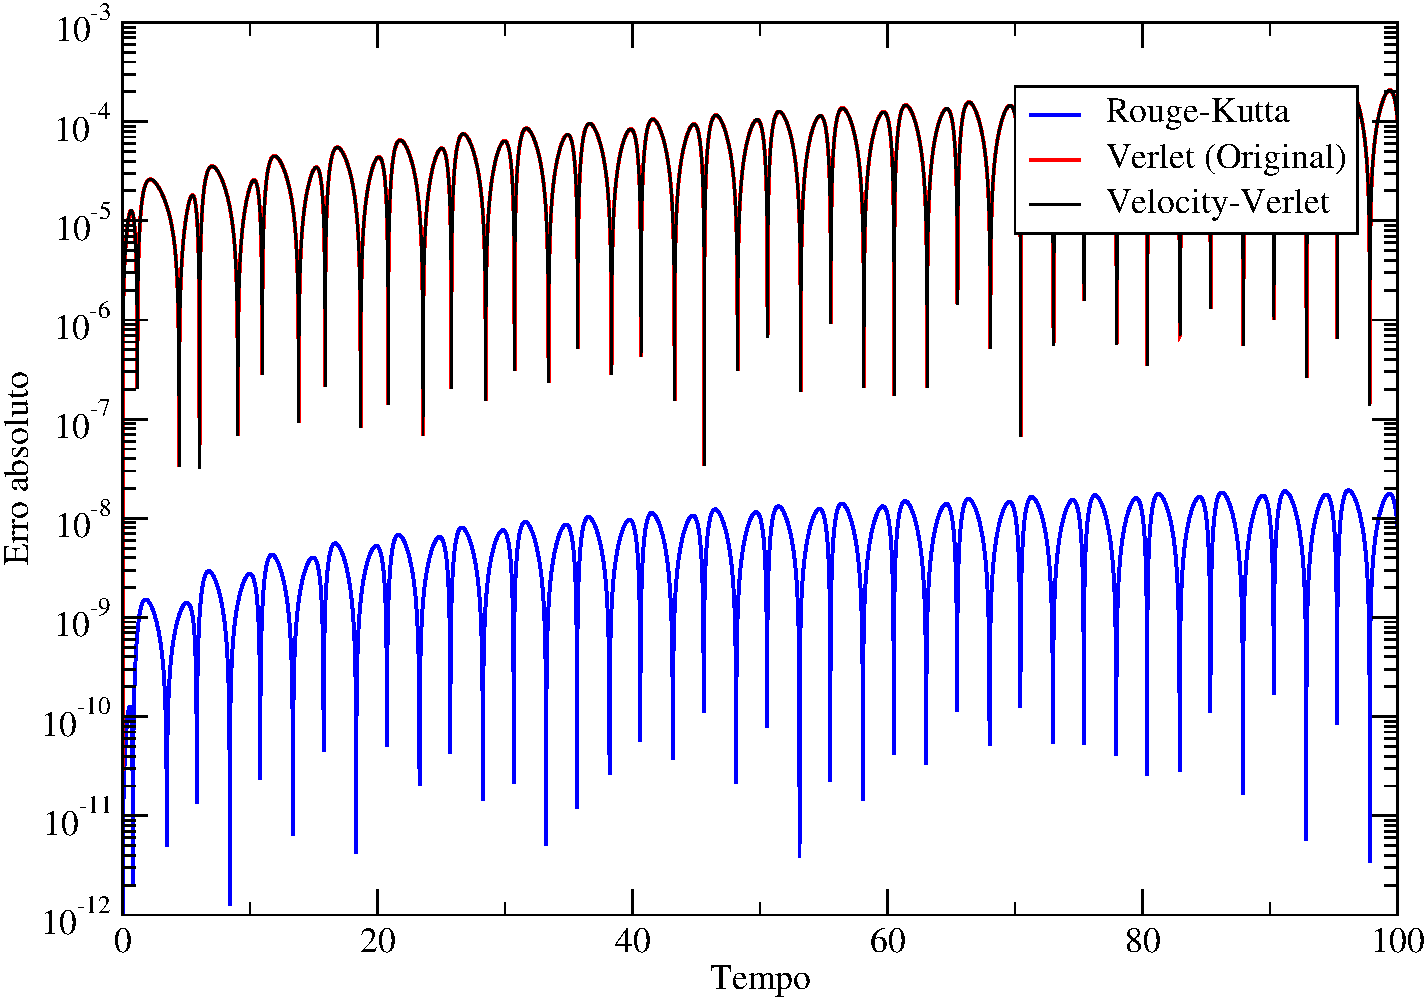
\includegraphics[width=0.42\textwidth]{erro.pdf}
\caption{Erro absoluto da posição para os três métodos.}
\label{4}
\end{figure}

Como pode ser visto, há pouquíssima diferença entre os métodos de Verlet (original) e Velocity-Verlet, ao passo que o método de Rouge-Kutta apresenta erros 4 ordens de grandeza menores.


\subsection*{b) }

Na Figura \ref{1} temos os resultados para a energia em função do tempo para os métodos de Rouge-Kutta, Verlet (original) e Velocity-Verlet, respectivamente. Nesta escala, apenas para o método Verlet original temos que a energia total não aparenta ser constante, devido aos erros do método. Este fato mostra que apesar do erro do método Velocity-Verlet não ser tão pequeno quanto o do método de Rouge-Kutta ele ainda se apresenta como uma aproximação melhor do que o método de Verlet original.


\begin{figure}[!htb]
\centering
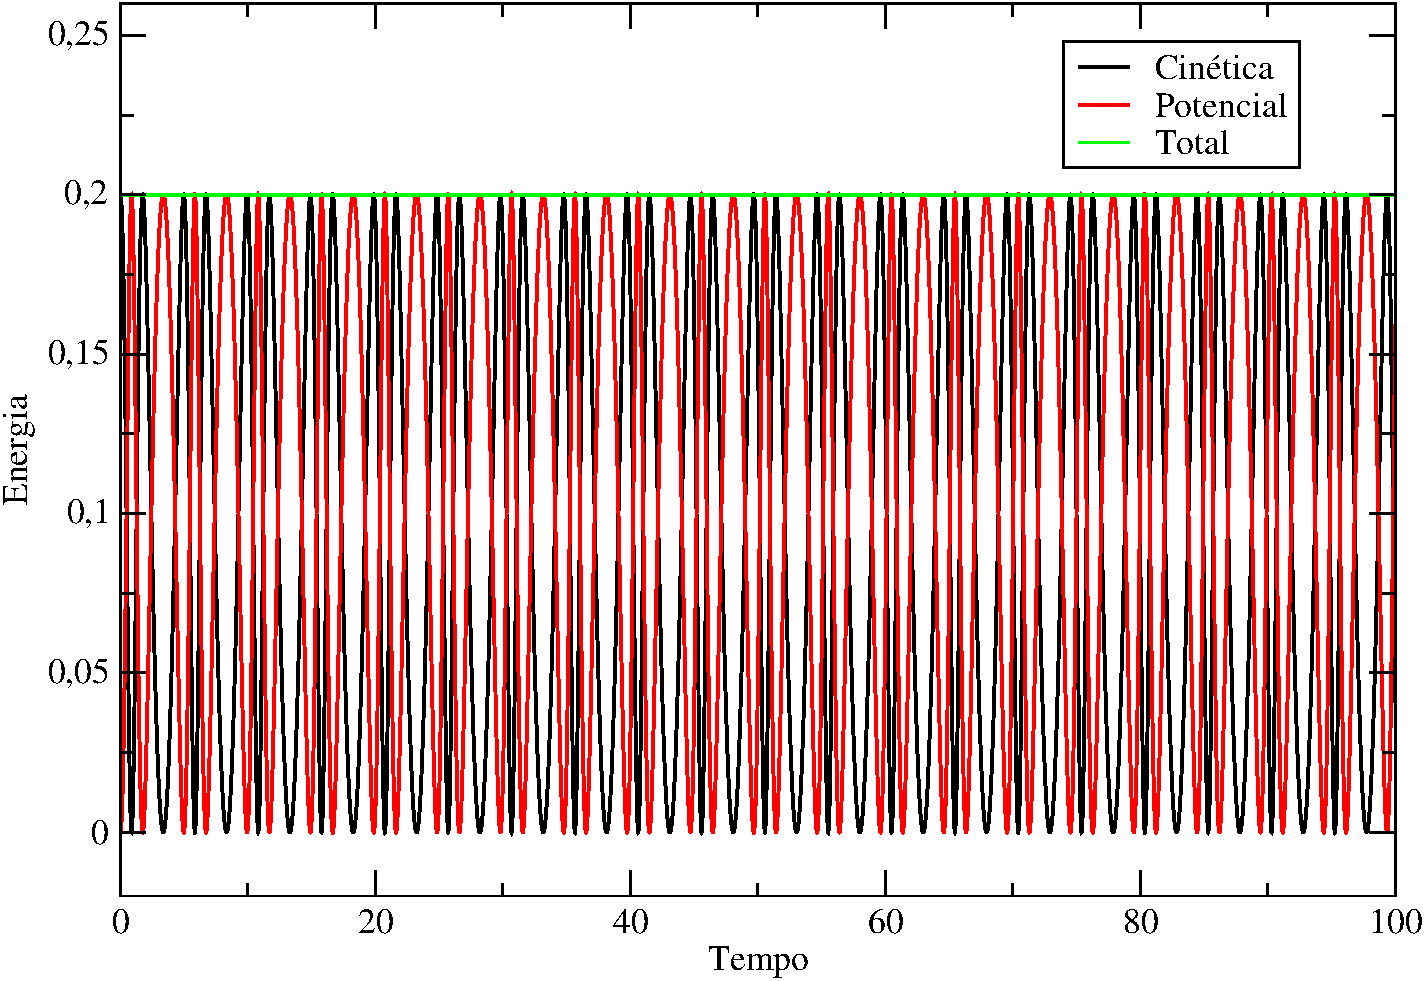
\includegraphics[width=0.32\textwidth]{rk.pdf}
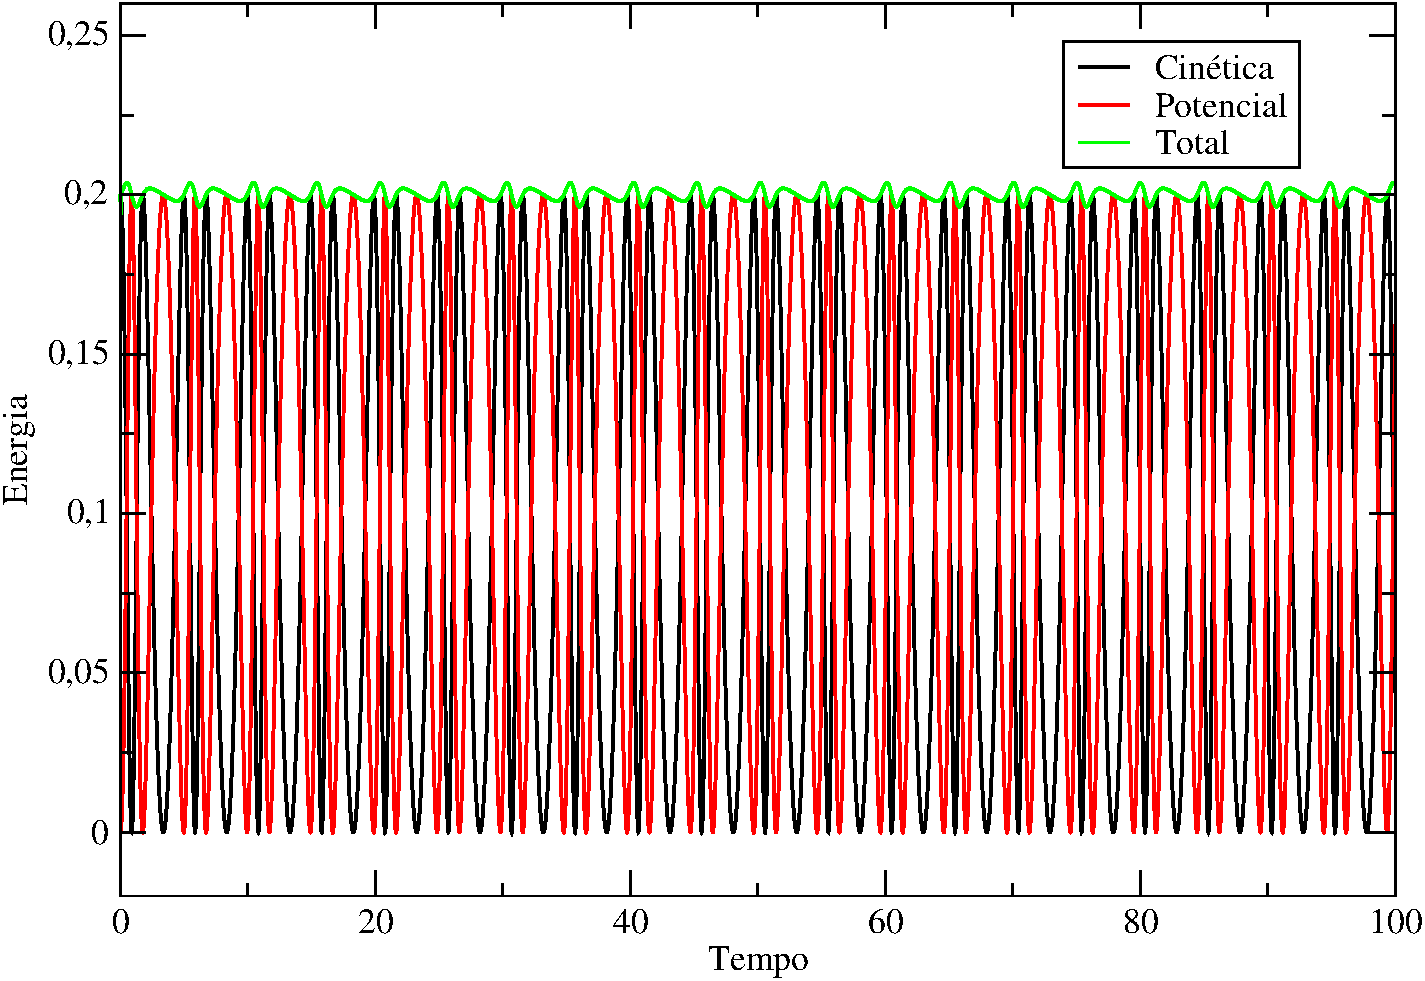
\includegraphics[width=0.32\textwidth]{VerletO.pdf}
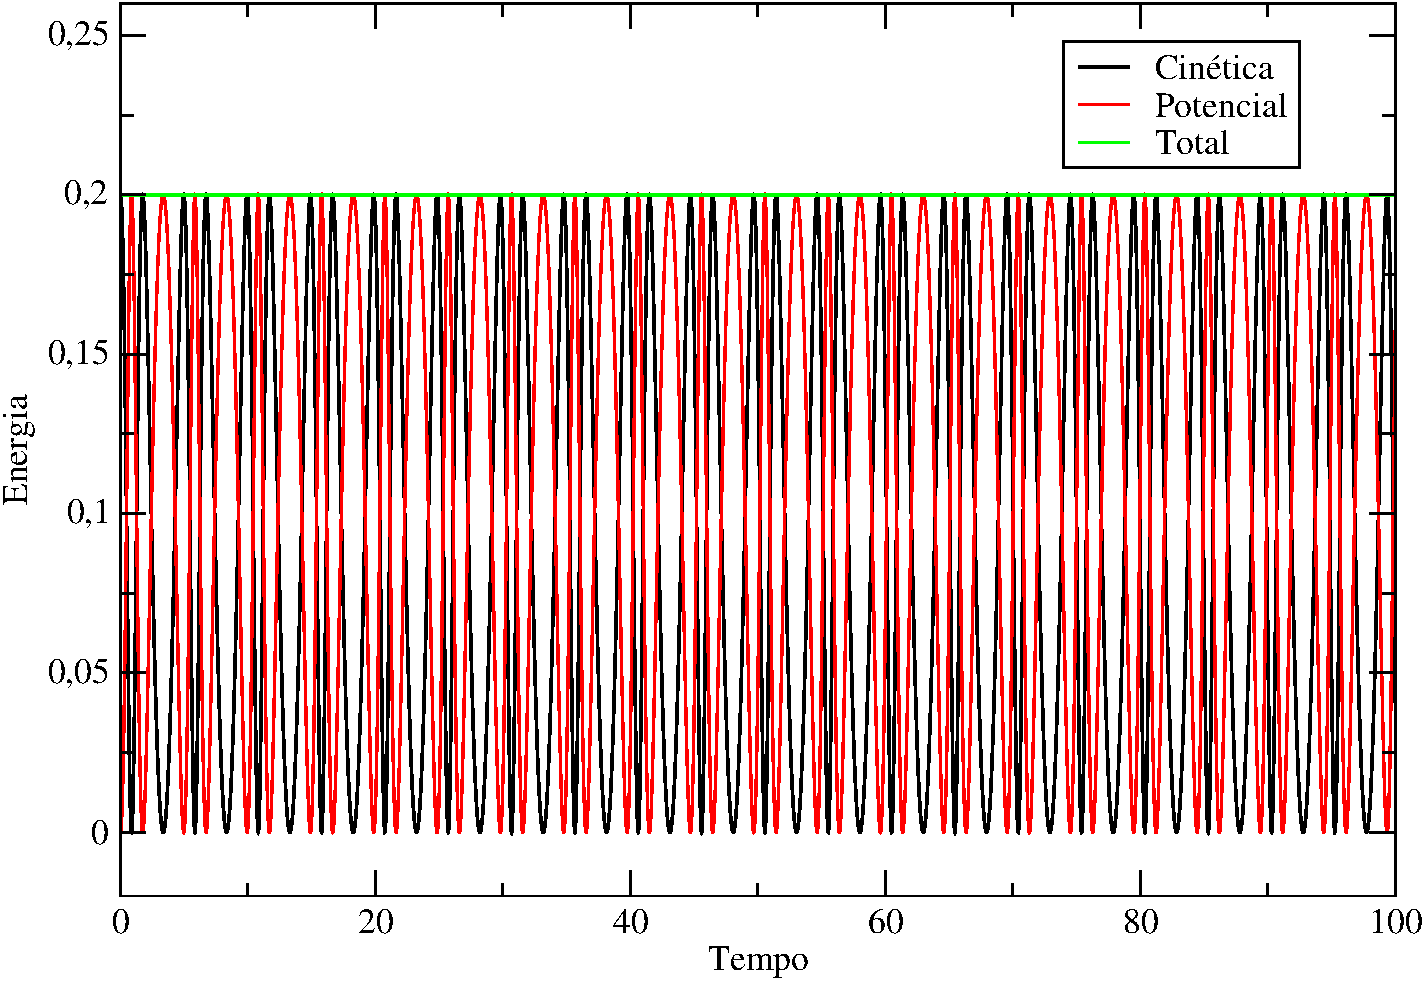
\includegraphics[width=0.32\textwidth]{VerletV.pdf}
\caption{Energia do sistema resolvida através do método de Rouge-Kutta, Velocity-Verlet e Verlet original, respectivamente.}
\label{1}
\end{figure}





\section*{Exercício 2}

\subsection*{a)}
A expressão da força é dada por:
\begin{equation}
F_k = -\frac{\partial U}{\partial u_k} = -\frac{\partial}{\partial u_k}\left[ \frac{k}{2}\sum_{j=1}^{N} (u_j - u_{j+1})^2 \right] 
\end{equation}

Que pode ser escrita da forma:
\begin{equation}
F_k = - k\sum_{j=1}^{N} (u_j - u_{j+1}) \left( \frac{\partial u_j}{\partial u_k} - \frac{\partial u_{j+1}}{\partial u_k}  \right)
\end{equation}

Os termos da forma $\partial u_j \setminus \partial u_k$ são deltas de Dirac $\delta_{j,k}$, de modo que temos:

\begin{equation*}
F_k = - k(u_j - u_{j+1}) \delta_{j,k} + k(u_j - u_{j+1}) \delta_{j+1,k} 
\end{equation*}

\begin{equation}
F_k = k(u_{k-1} - 2u_{k} + u_{k+1})  
\end{equation}

Os casos k = 1 e k = N são diferentes e precisamos recorrer às condições de contorno:

$\begin{cases} 
F_1 = k (u_{N} - 2u_1 + u_2) \\ 
F_N = k (u_{N-1} - 2u_N + u_1)
\end{cases} $

\subsection*{b)}

A energia do oscilador pode ser vista na Figura \ref{2b1}. Como esperado, a energia total é constante.
\begin{figure}[!htb]
\centering
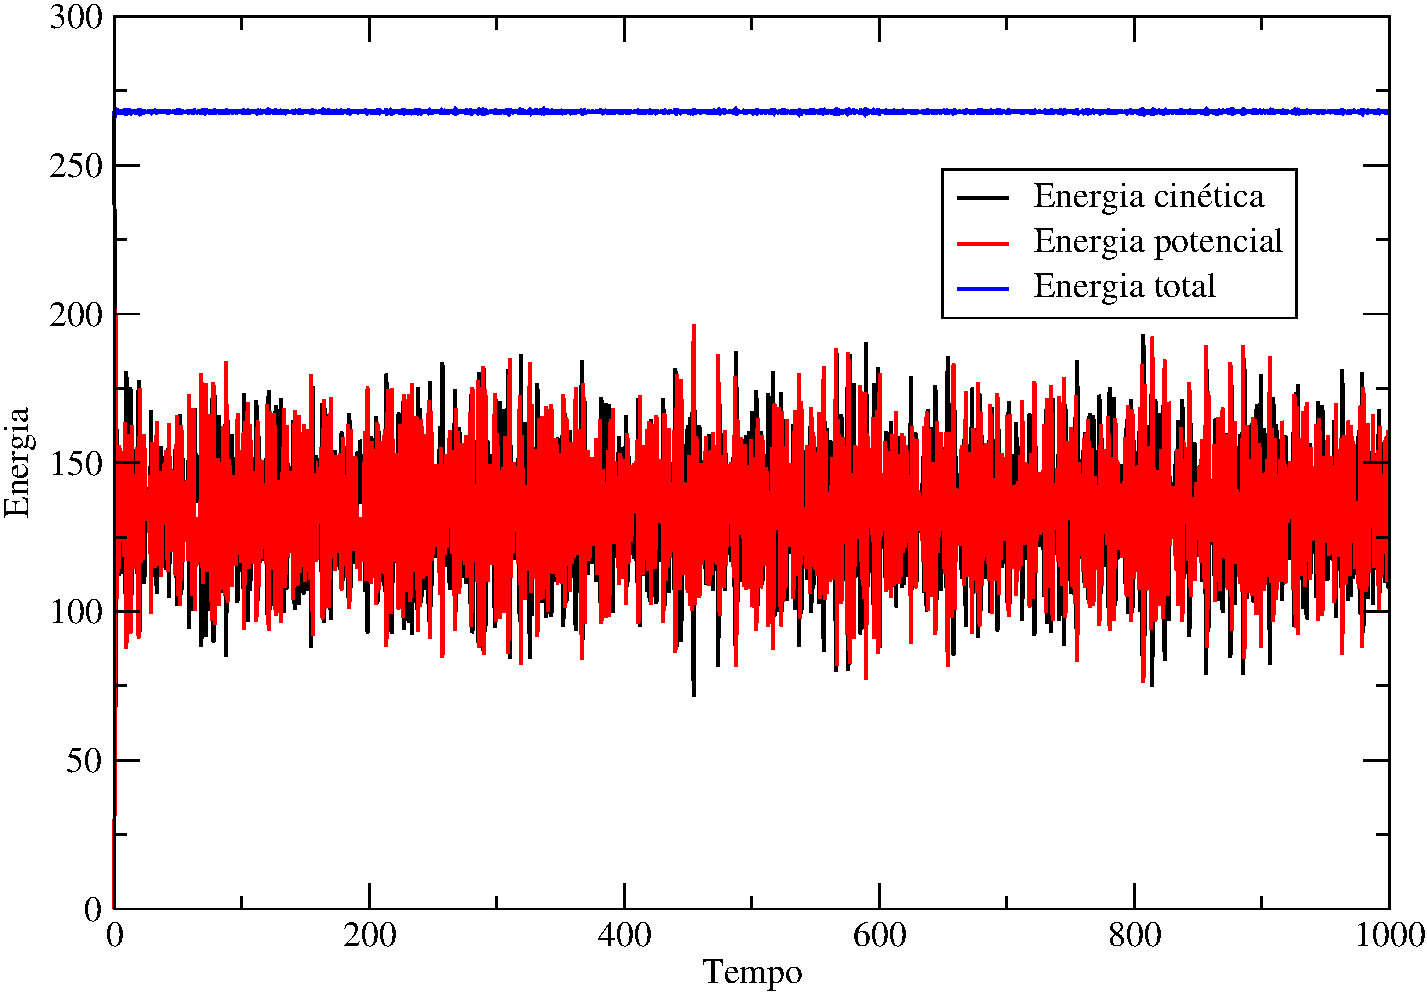
\includegraphics[width=0.4\textwidth]{energia.pdf}
\caption{Energias cinética, potencial e total para as condições iniciais 1.}
\label{2b1}
\end{figure}

Na Figura \ref{2b2} podemos ver o momento linear total e a temperatura do sistema. Vemos que para esta configuração inicial o momento total parece oscilar em torno do zero e a temperatura oscila em torno de T = 2.

\begin{figure}[!htb]
\centering
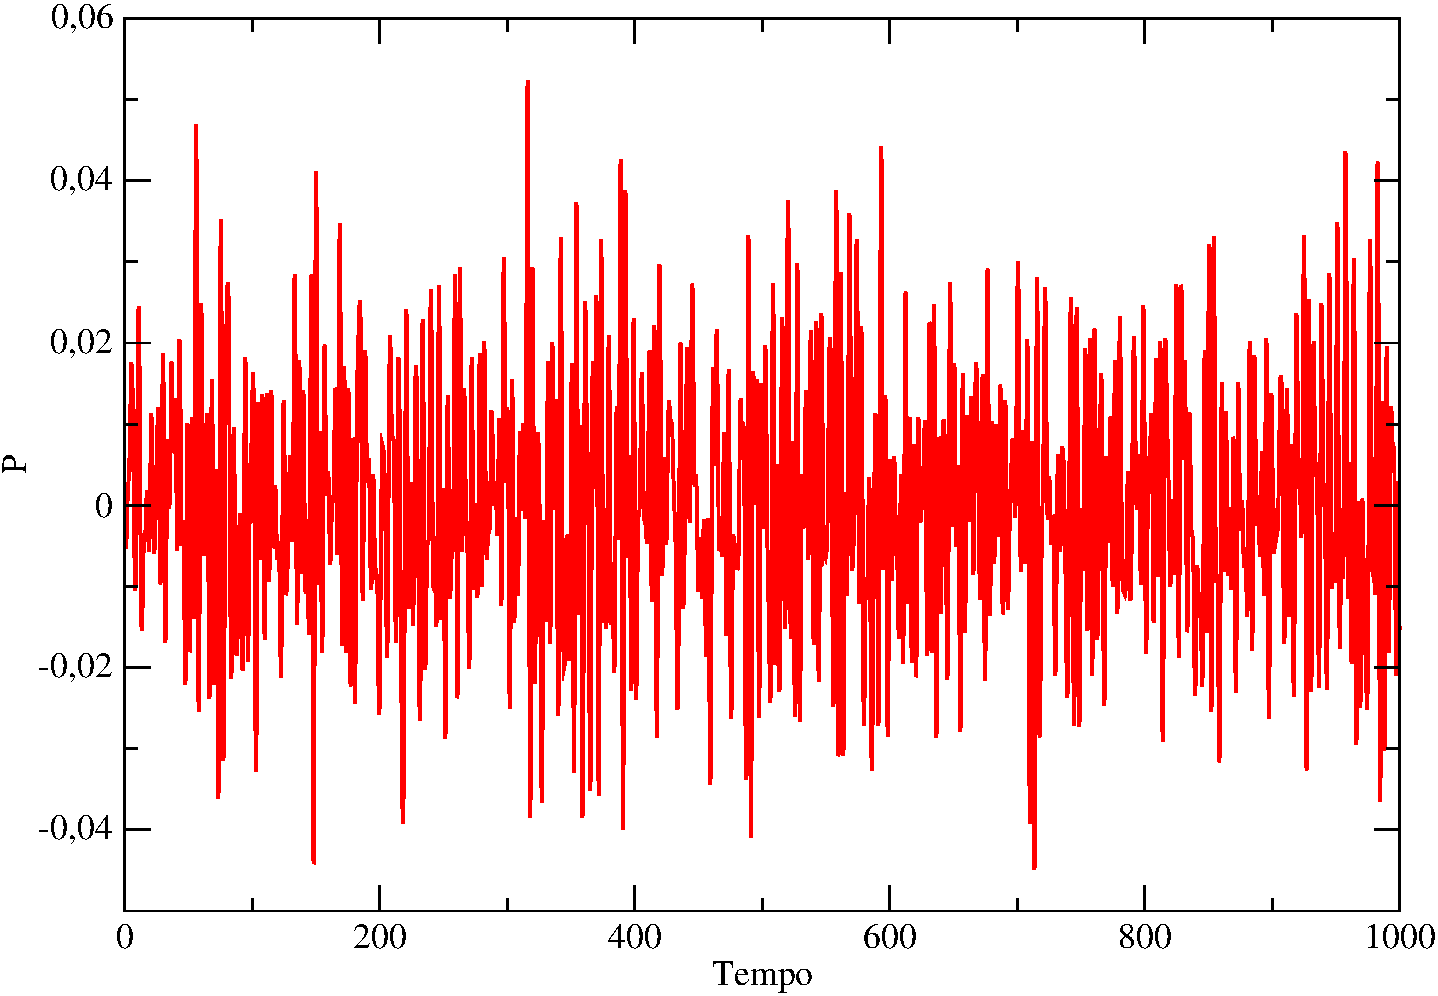
\includegraphics[width=0.4\textwidth]{P.pdf}
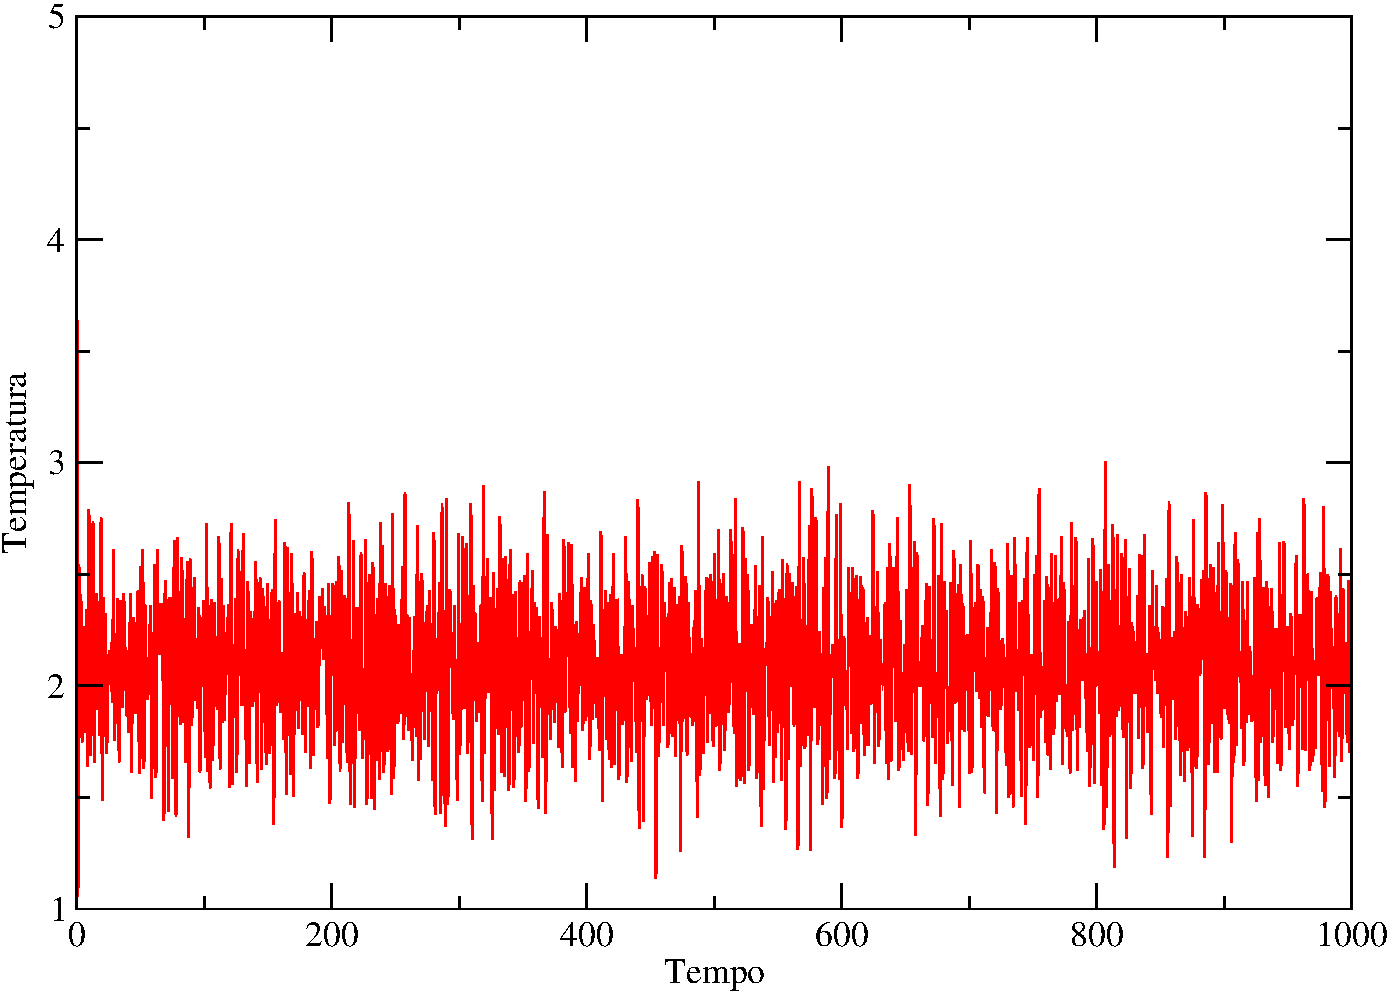
\includegraphics[width=0.4\textwidth]{temp.pdf}
\caption{Momento linear total (esquerda) e temperatura (direita) para as condições iniciais 1.}
\label{2b2}
\end{figure}


\subsection*{c)}

A energia do oscilador para as condições iniciais 2 pode ser vista na Figura \ref{2c1}. Como esperado, a energia total é constante; além disso, possui um valor muito parecido com o das condições iniciais anteriores. Na Figura \ref{2c2} podemos ver o momento linear total e a temperatura do sistema, que  oscilam em torno de $P = -19.37$ e T = 2.

\begin{figure}[!htb]
\centering
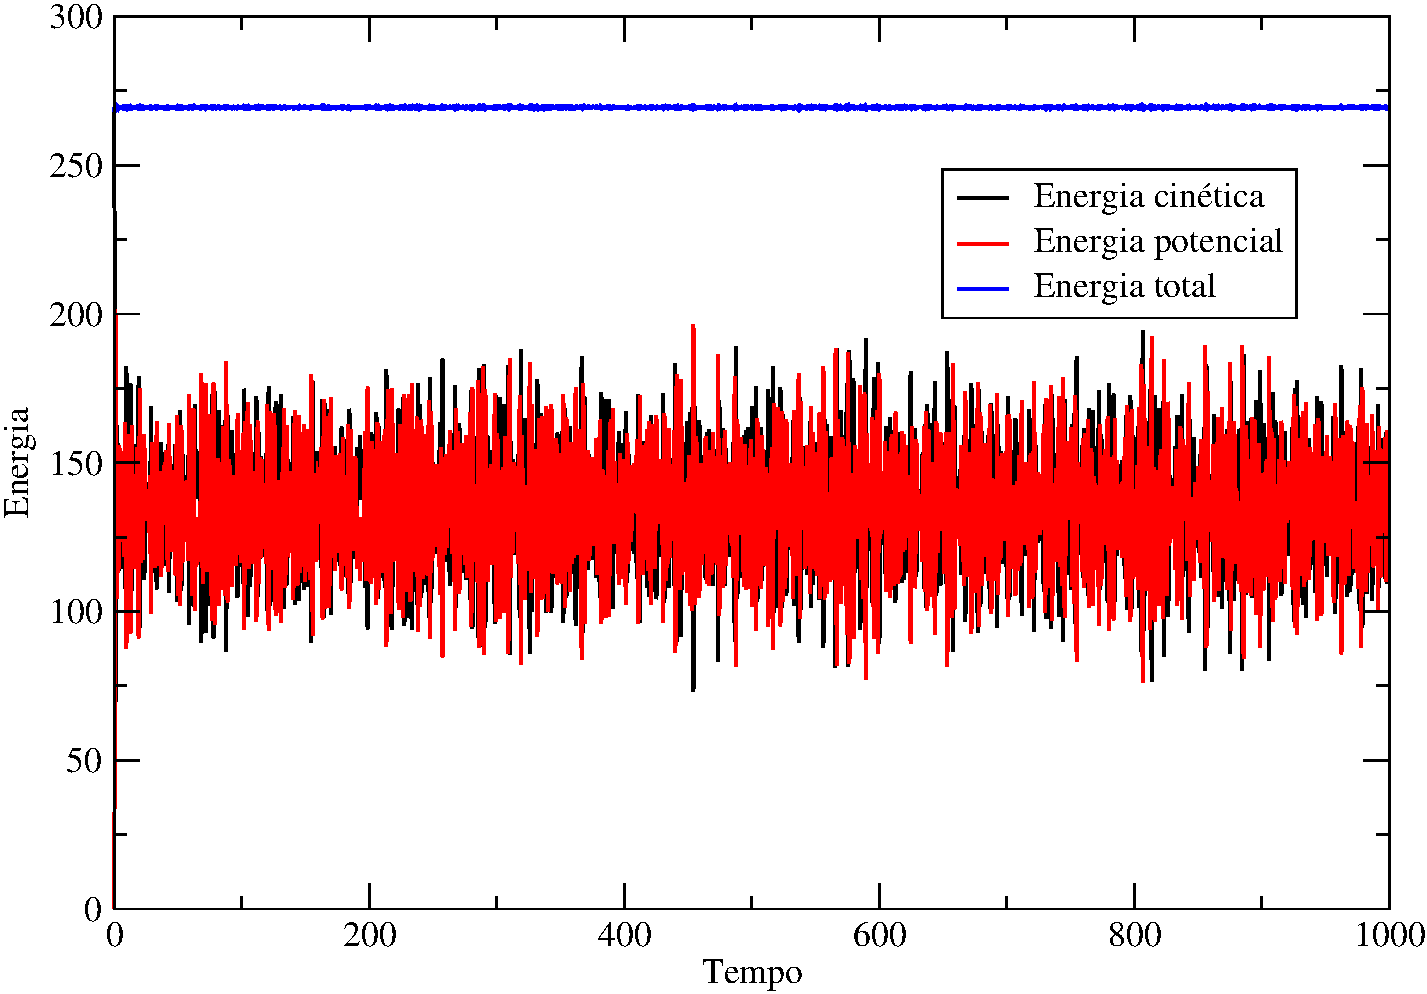
\includegraphics[width=0.447\textwidth]{energia2.pdf}
\caption{Energias cinética, potencial e total para as condições iniciais 2.}
\label{2c1}
\end{figure}



\begin{figure}[!htb]
\centering
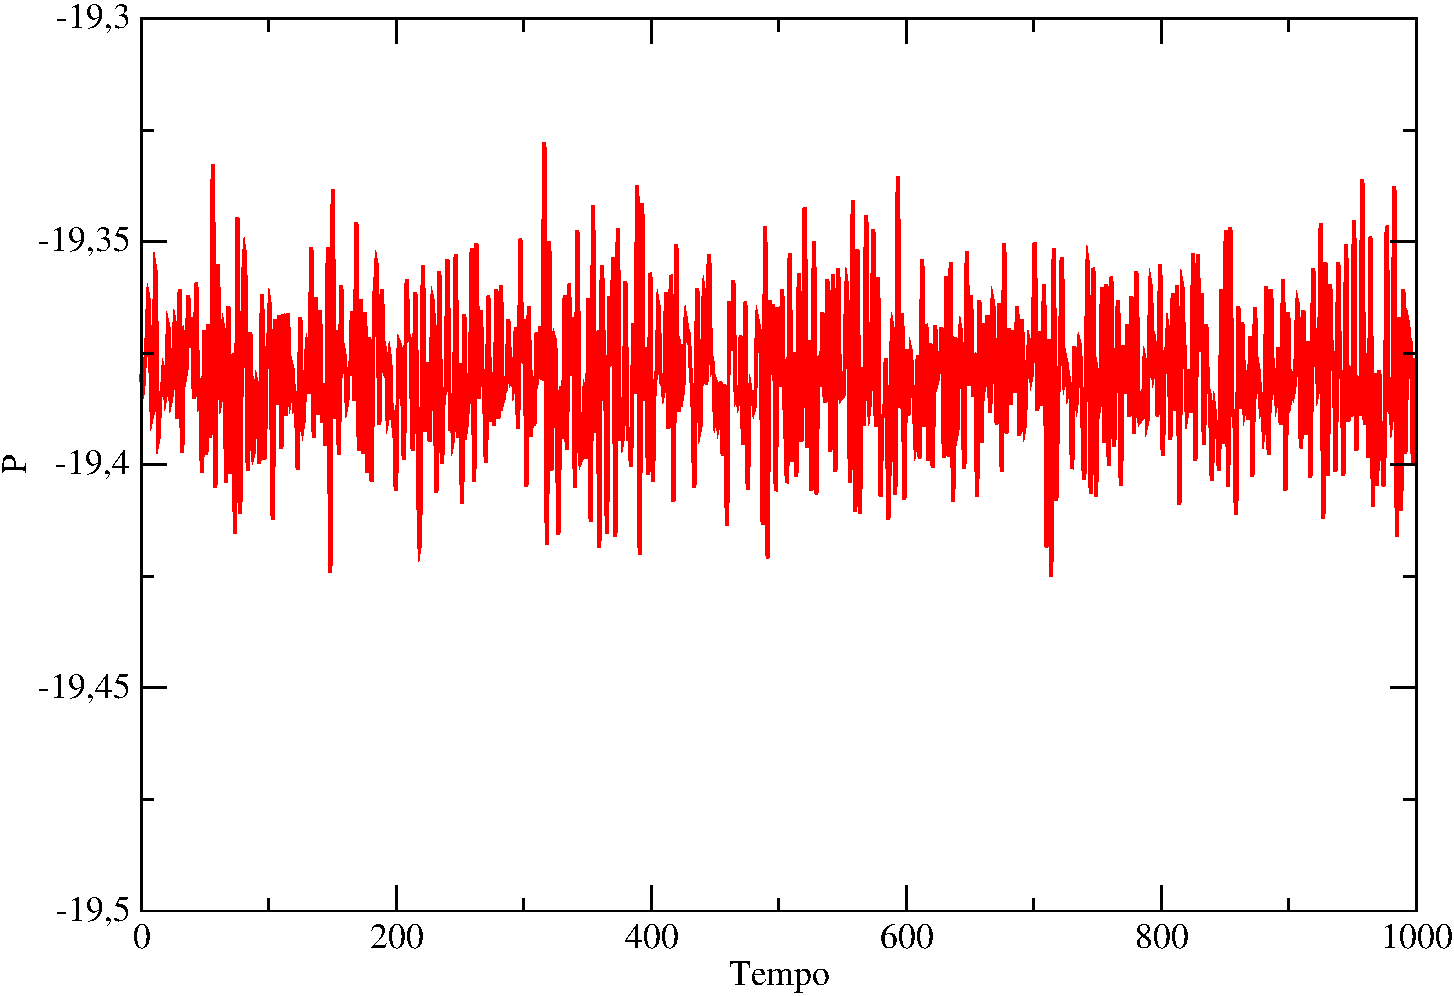
\includegraphics[width=0.4\textwidth]{p2.pdf}
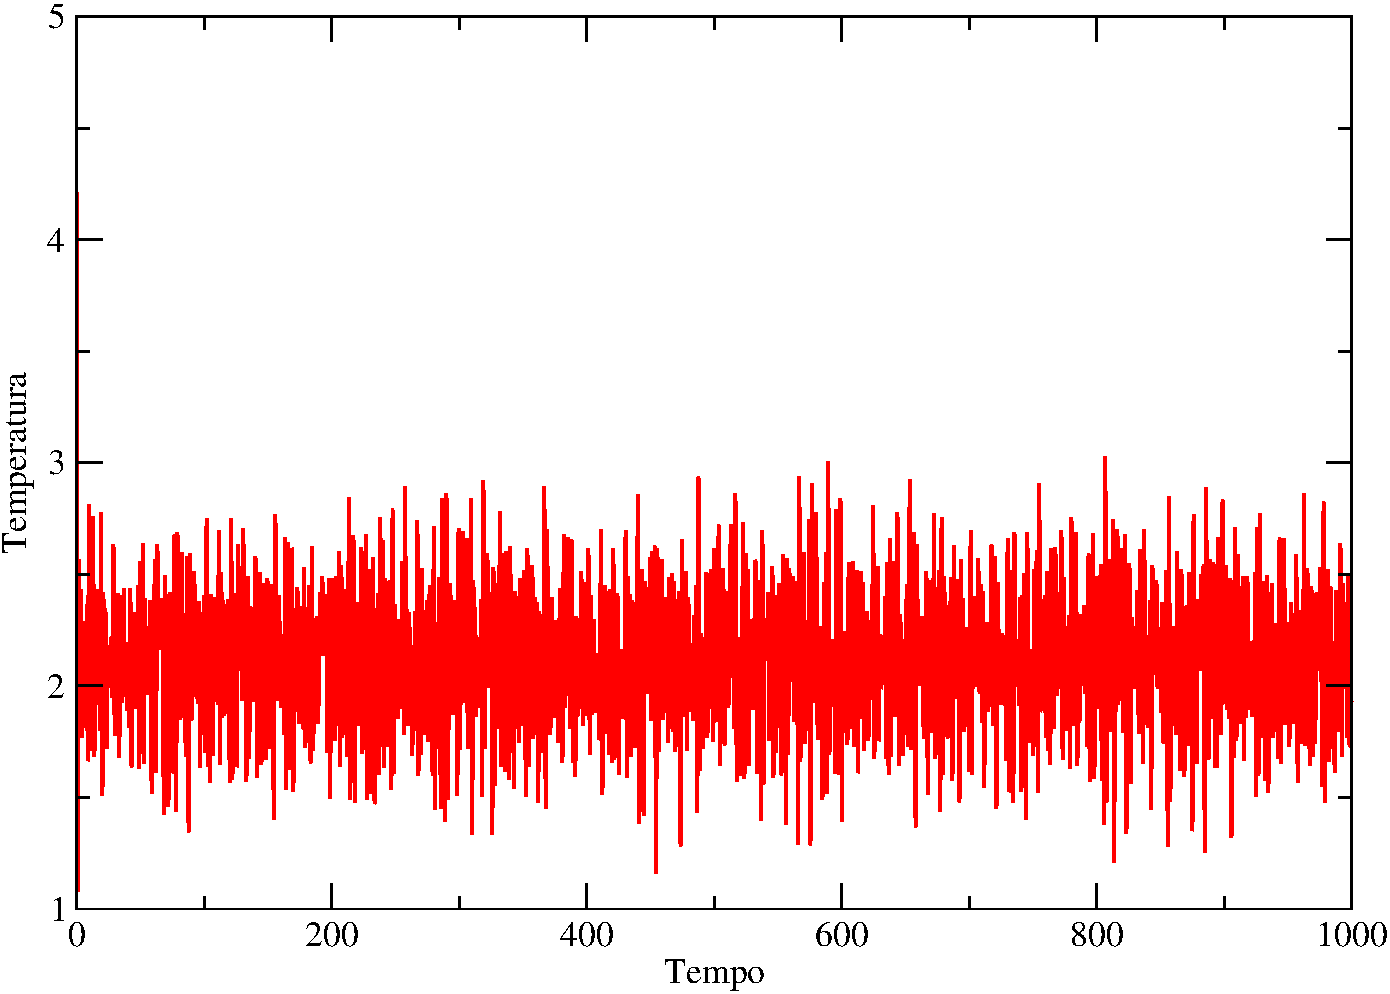
\includegraphics[width=0.4\textwidth]{temp2.pdf}
\caption{Momento linear total (esquerda) e temperatura (direita) para as condições iniciais 2.}
\label{2c2}
\end{figure}

\subsection*{d)}

Na Figura \ref{2d1} temos o gráfico da energia total por oscilador (esquerda) e temperatura (direita) para cada um dos dois subsistemas. Como pode ser visto temos que tanto a energia por oscilador quanto a temperatura tendem a convergir para 2. Este resultado é esperado visto que o fato destes dois subsistemas estarem em contato significa que eles eventualmente devem atingir o equilibrio térmico. Além disso, o teorema da equipartição de energia prevê que a energia média por oscilador deve ser $E = k_b T$. Como em nossa simulação $k_b = 1$, temos que tanto a energia por oscilador quanto a temperatura devem convergir para o mesmo valor.

\begin{figure}[!htb]
\centering
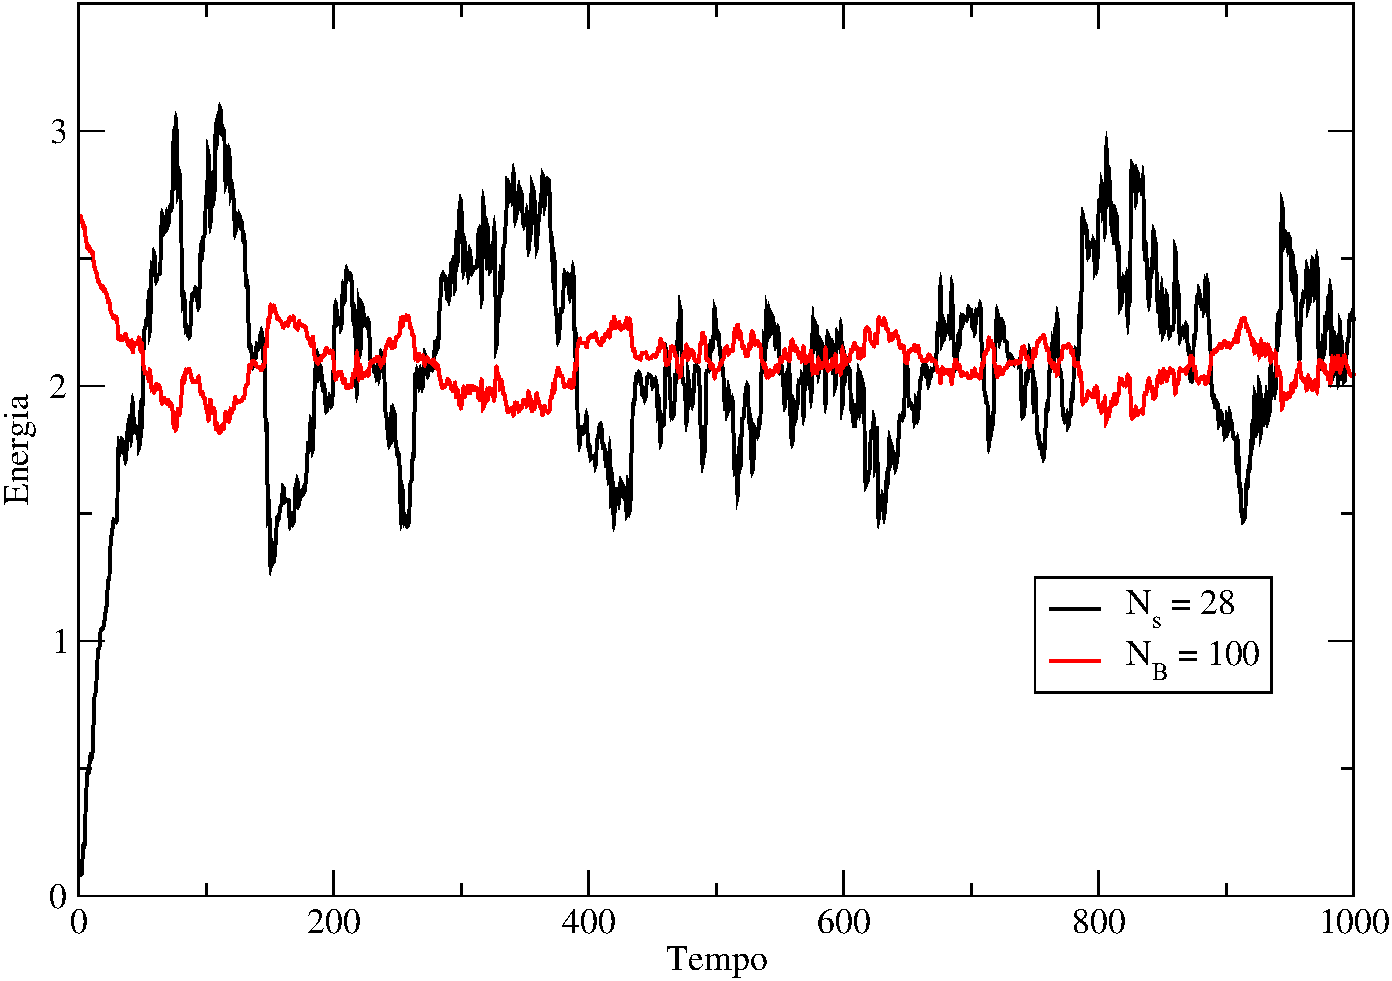
\includegraphics[width=0.4\textwidth]{energia2d.pdf}
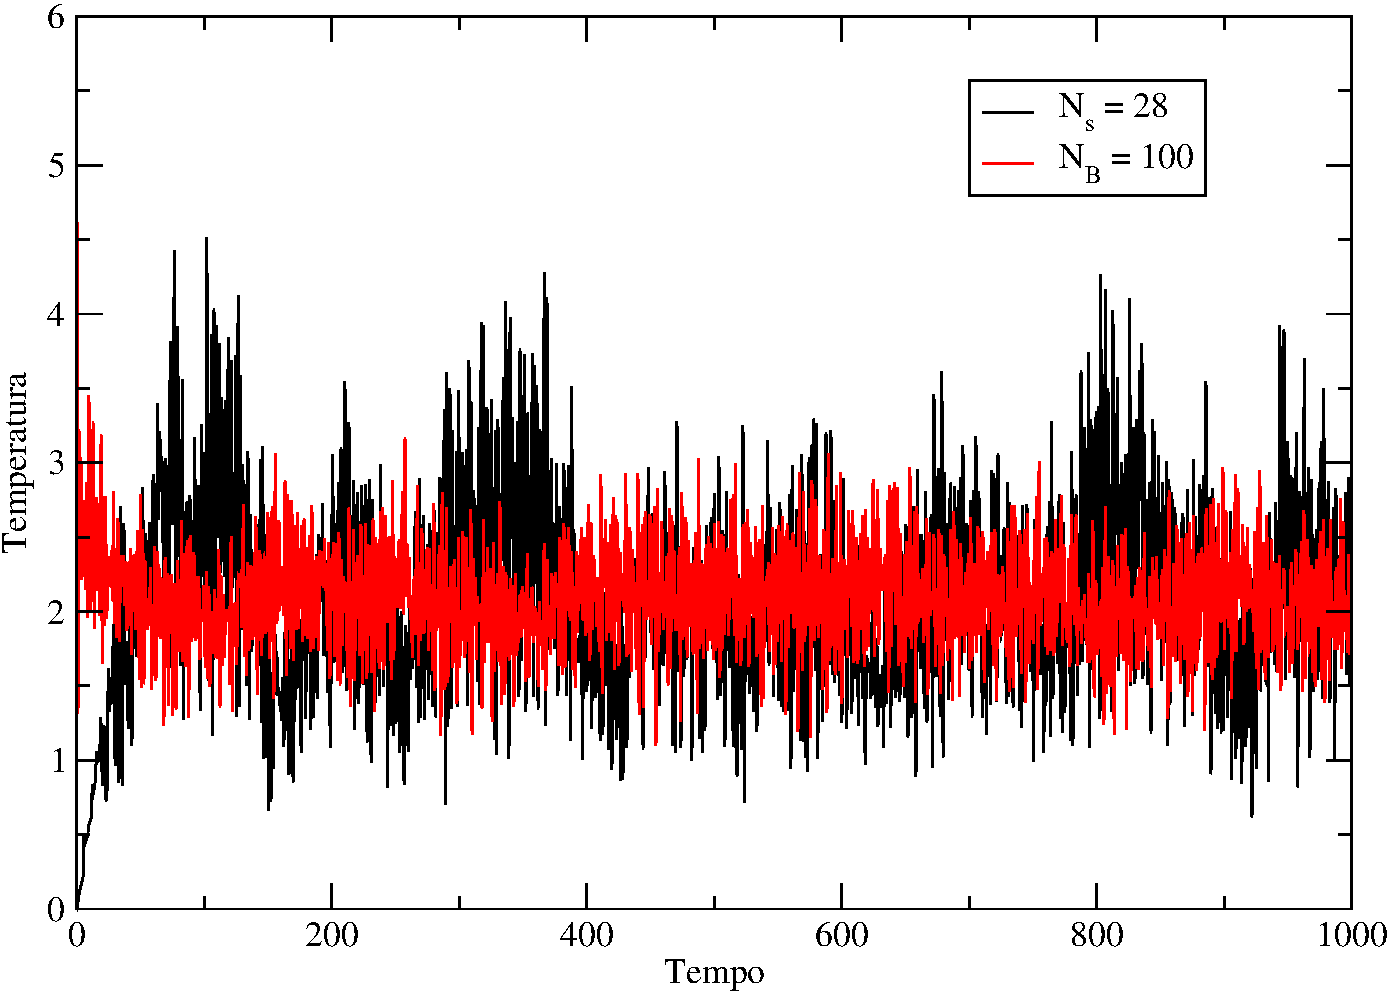
\includegraphics[width=0.4\textwidth]{temp2d.pdf}
\caption{Energia por oscilador (esquerda) e temperatura (direita).}
\label{2d1}
\end{figure}

\subsection*{e)}
O teorema do Virial afirma que para um potencial central da forma $V(r) = A/r^{n}$ temos[1]:

\begin{equation}
<T> =-\frac{n}{2} <V>
\end{equation}

Para o nosso caso temos $ n = -2$, de modo que:
\begin{equation}
<T> = <V>
\end{equation}

Nos gráficos a seguir temos a comparação entre as condições iniciais 1 e 3. Na Figura \ref{2e1} temos a energia por oscilador do subsistema B e do subsistema S em função do tempo para as duas condições iniciais. 

\begin{figure}[!htb]
\centering
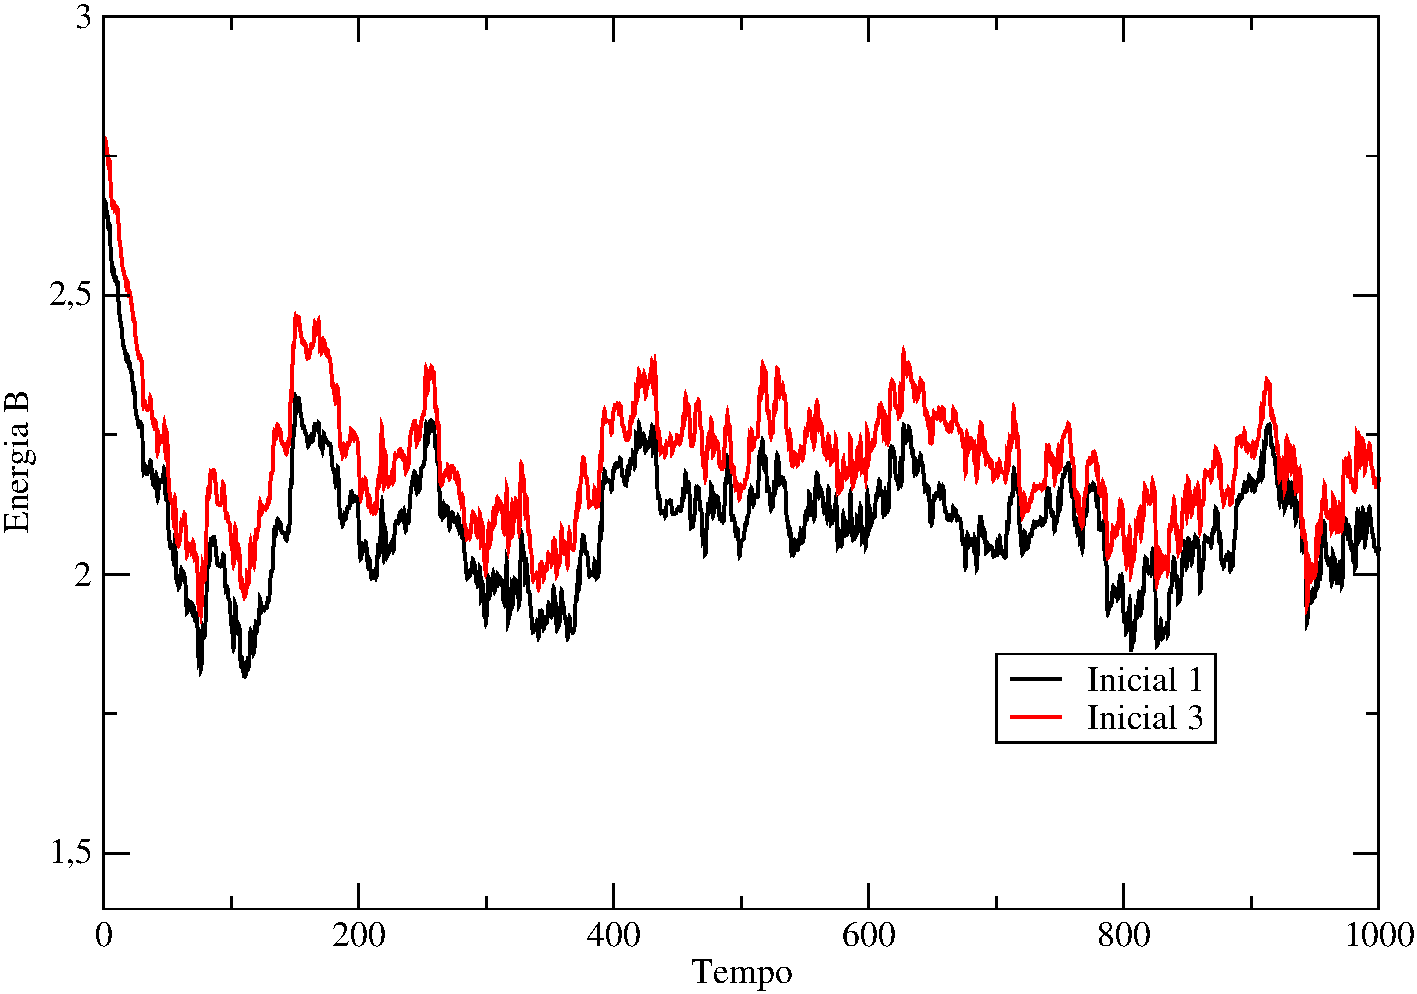
\includegraphics[width=0.4\textwidth]{ETB.pdf}
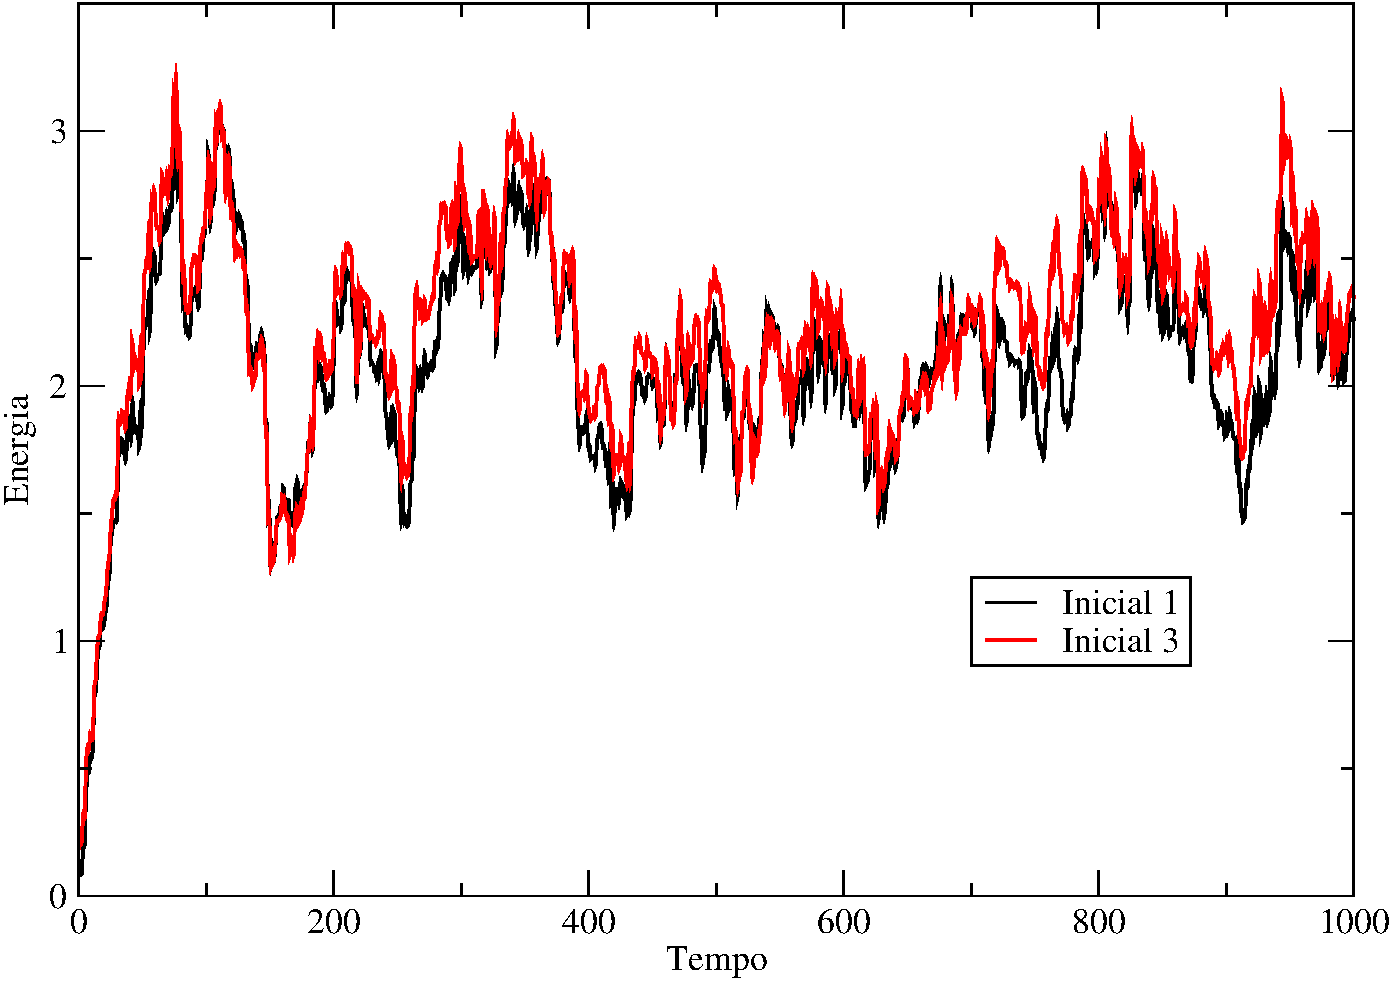
\includegraphics[width=0.4\textwidth]{ETS.pdf}
\caption{Energia por oscilador do subsistema B (esquerda) e do subsistema S (direita).}
\label{2e1}
\end{figure}

Na Figura \ref{2e2} temos a comparação entre as temperaturas para os subsistemas B e S. Assim como na Figura \ref{2e1} temos que os dois subsistemas se comportam de maneira muito semelhante e os gráficos acabam se interpondo.

\begin{figure}[!htb]
\centering
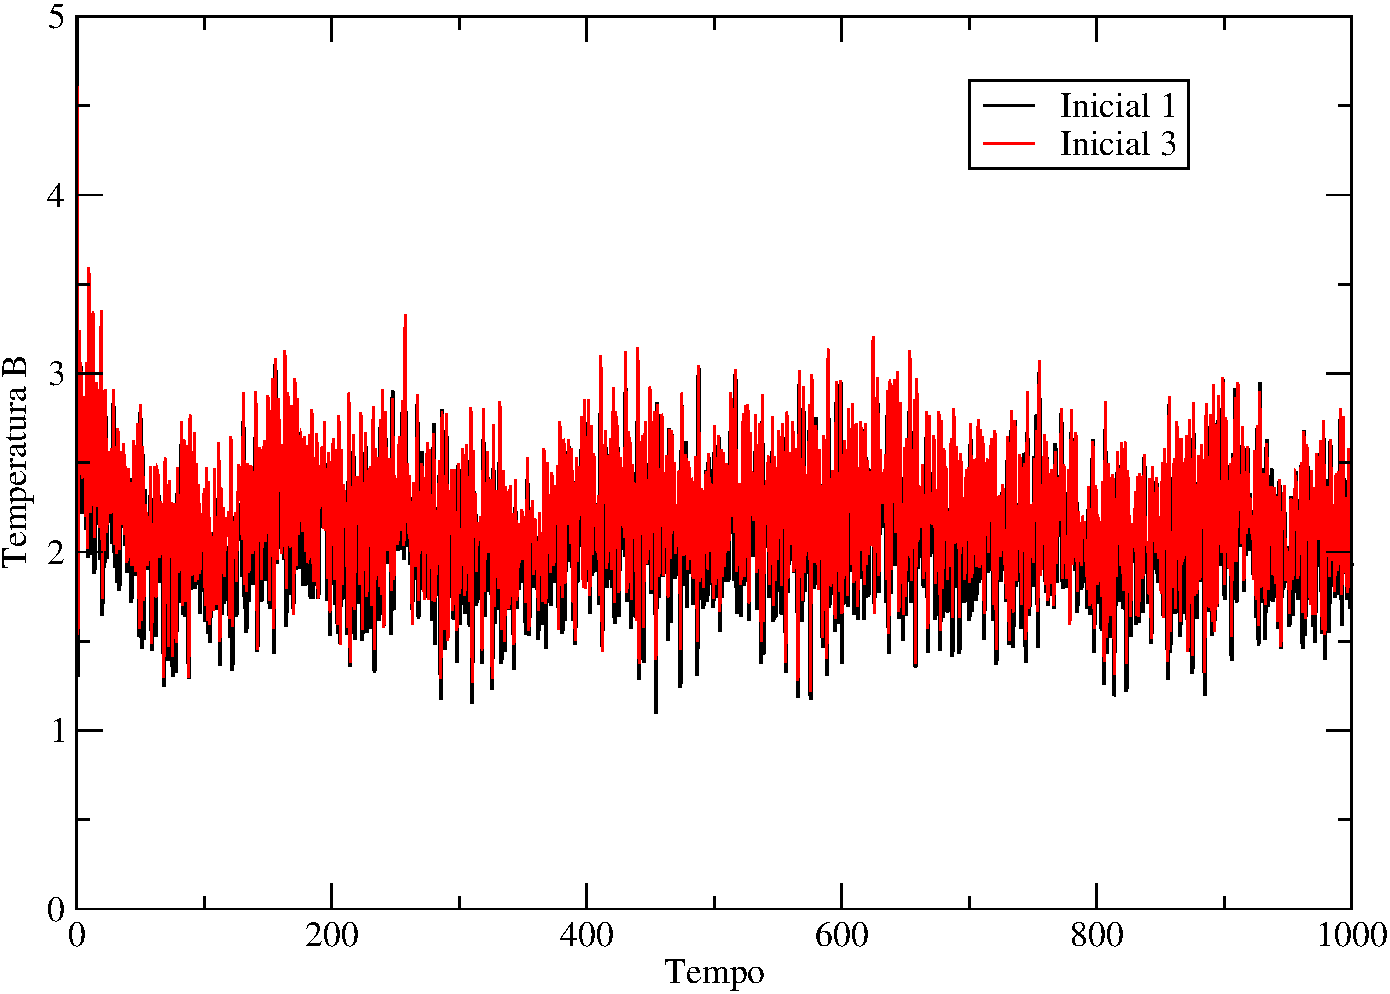
\includegraphics[width=0.4\textwidth]{tempB.pdf}
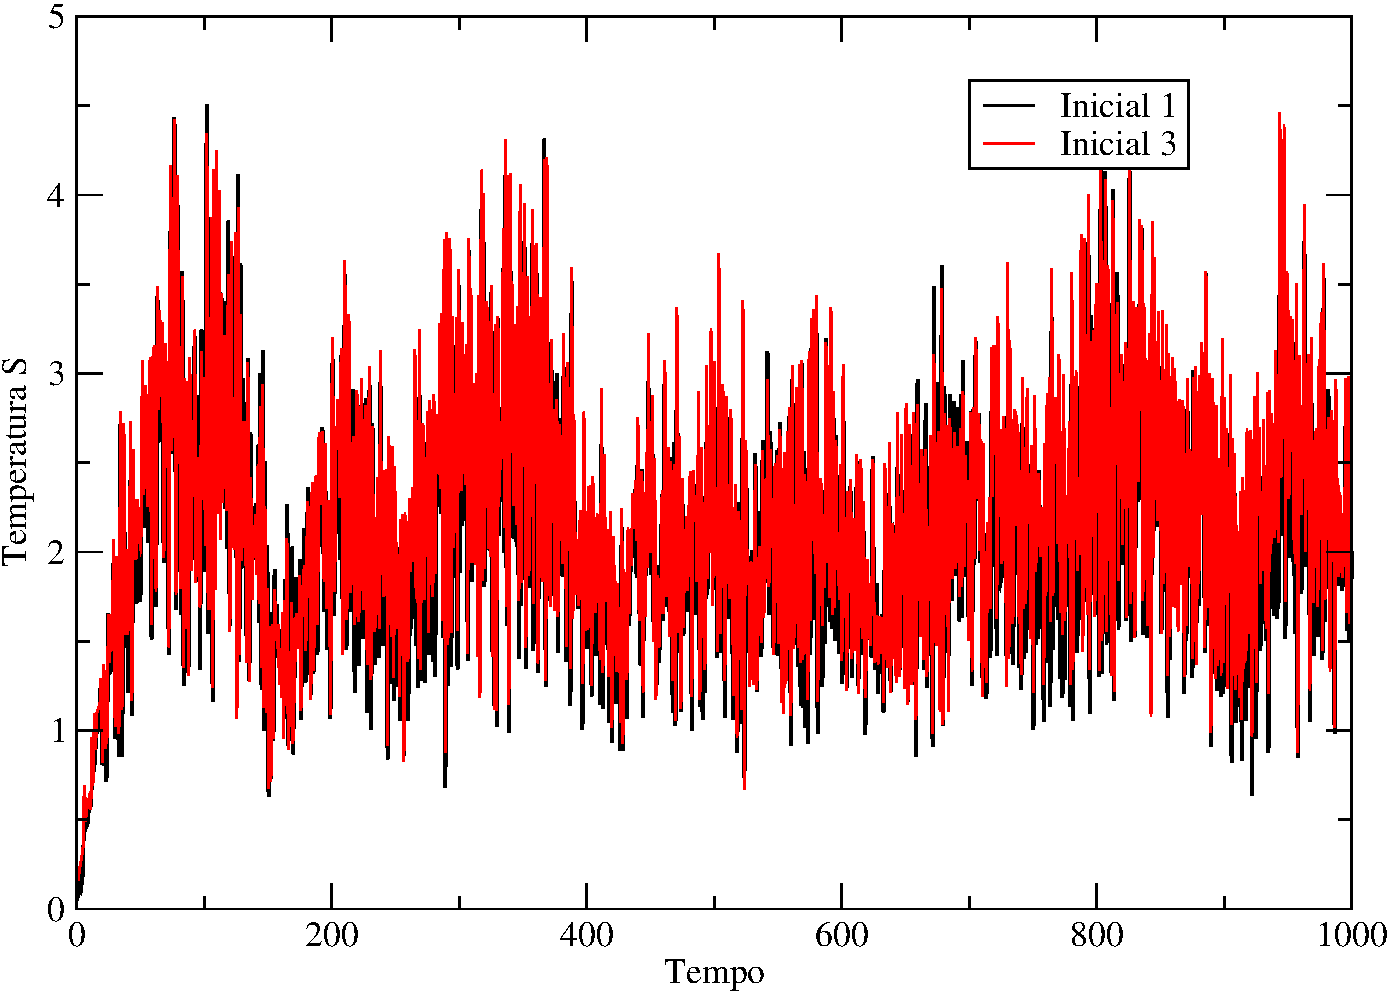
\includegraphics[width=0.4\textwidth]{tempS.pdf}
\caption{Temperatura do subsistema B (esquerda) e do subsistema S (direita).}
\label{2e2}
\end{figure}


\section*{Exercício 3}
\subsection*{a)}
Devido aos números envolvidos no cálculo serem muito grandes foram utilizadas as unidades $10^6$ km para posição, anos para o tempo e $10^6$ km/ano para a velocidade. Além disto, como a constante G sempre aparece multiplicada por $M_s$ foi criado uma constante auxiliar que é o produto das duas em nosso sistema de unidades, ou seja, $GM_s \approx 1.33 \times 10^8  (10^6 km)^3kg^{-1}anos^{-2}$. Para escolher o valor de $\Delta t$ foram feitas diversas simulações e verificado que para valores de $\Delta t$ relativamente grandes a órbita não se fechava, o que não acontecia com valores menores. Assim sendo, foi escolhido um valor de $\Delta t$ tal que visualmente os gráficos gerados não apresentassem ruídos e de modo que o tempo total de simulação não ultrapassasse 1 segundo.

Na Figura \ref{3a3} temos a coordenada Y em funçao da coordenada X e a componente y da velocidade em função da componente x da velocidade.


\begin{figure}[!htb]
\centering
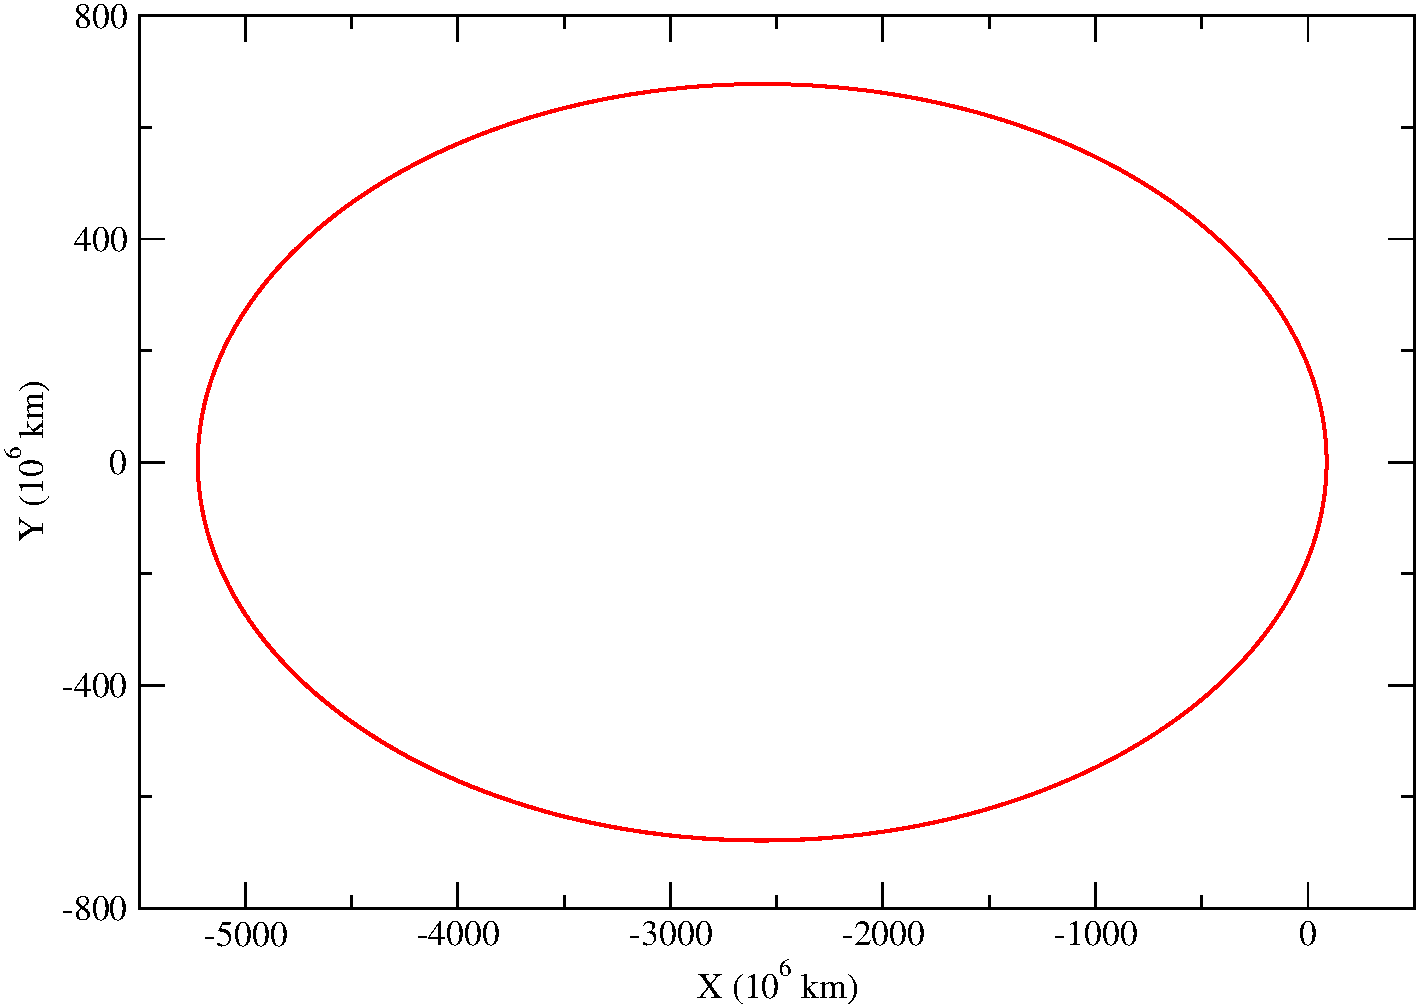
\includegraphics[width=0.447\textwidth]{xy.pdf}
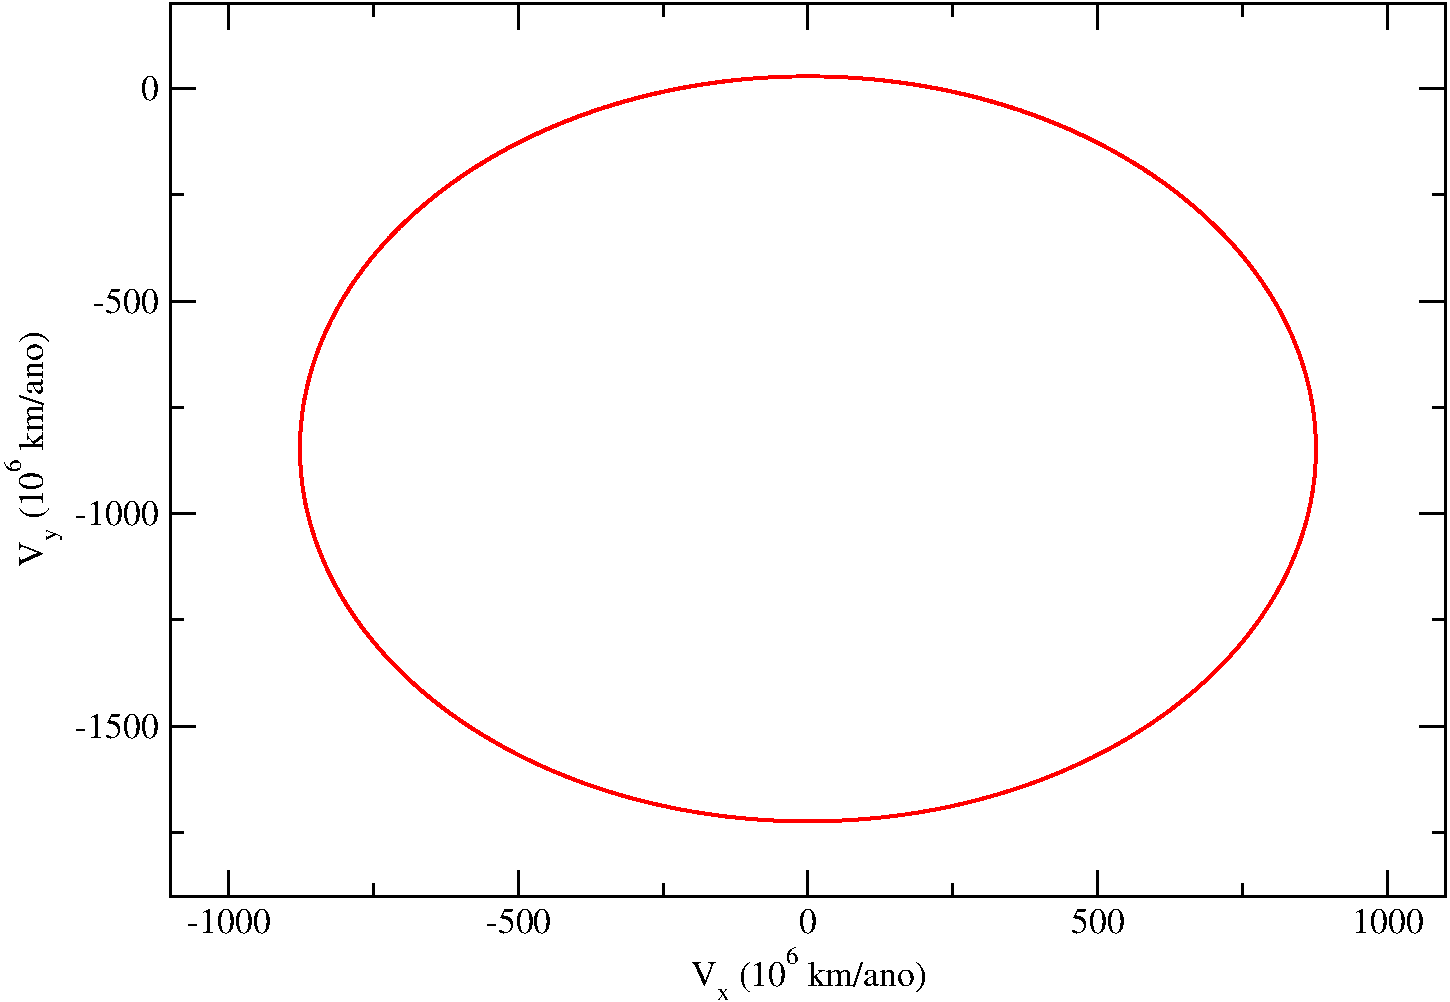
\includegraphics[width=0.447\textwidth]{vxvy.pdf}
\caption{Coordenada Y em função da coordenada X (esquerda) e componente Y da velocidade em função da componente X da velocidade (direita).}
\label{3a3}
\end{figure}


\subsection*{b)}
Na Figura \ref{3b1} temos as energias cinética, potencial e total. Como esperado, a energia total do sistema é constante.
\begin{figure}[!htb]
\centering
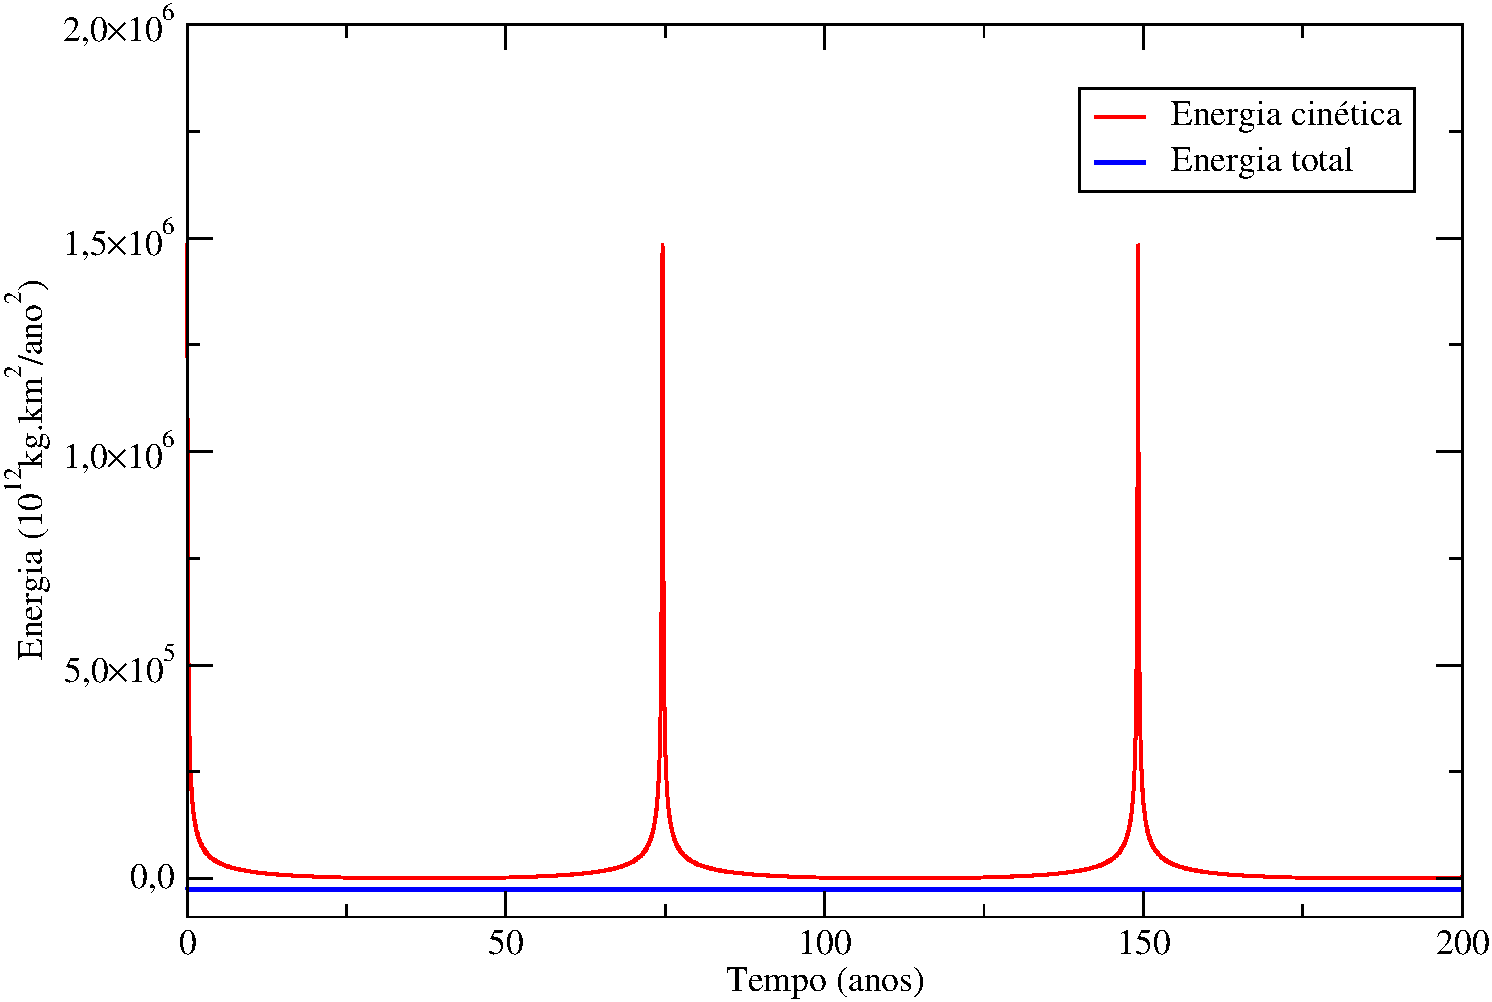
\includegraphics[width=0.447\textwidth]{K.pdf}
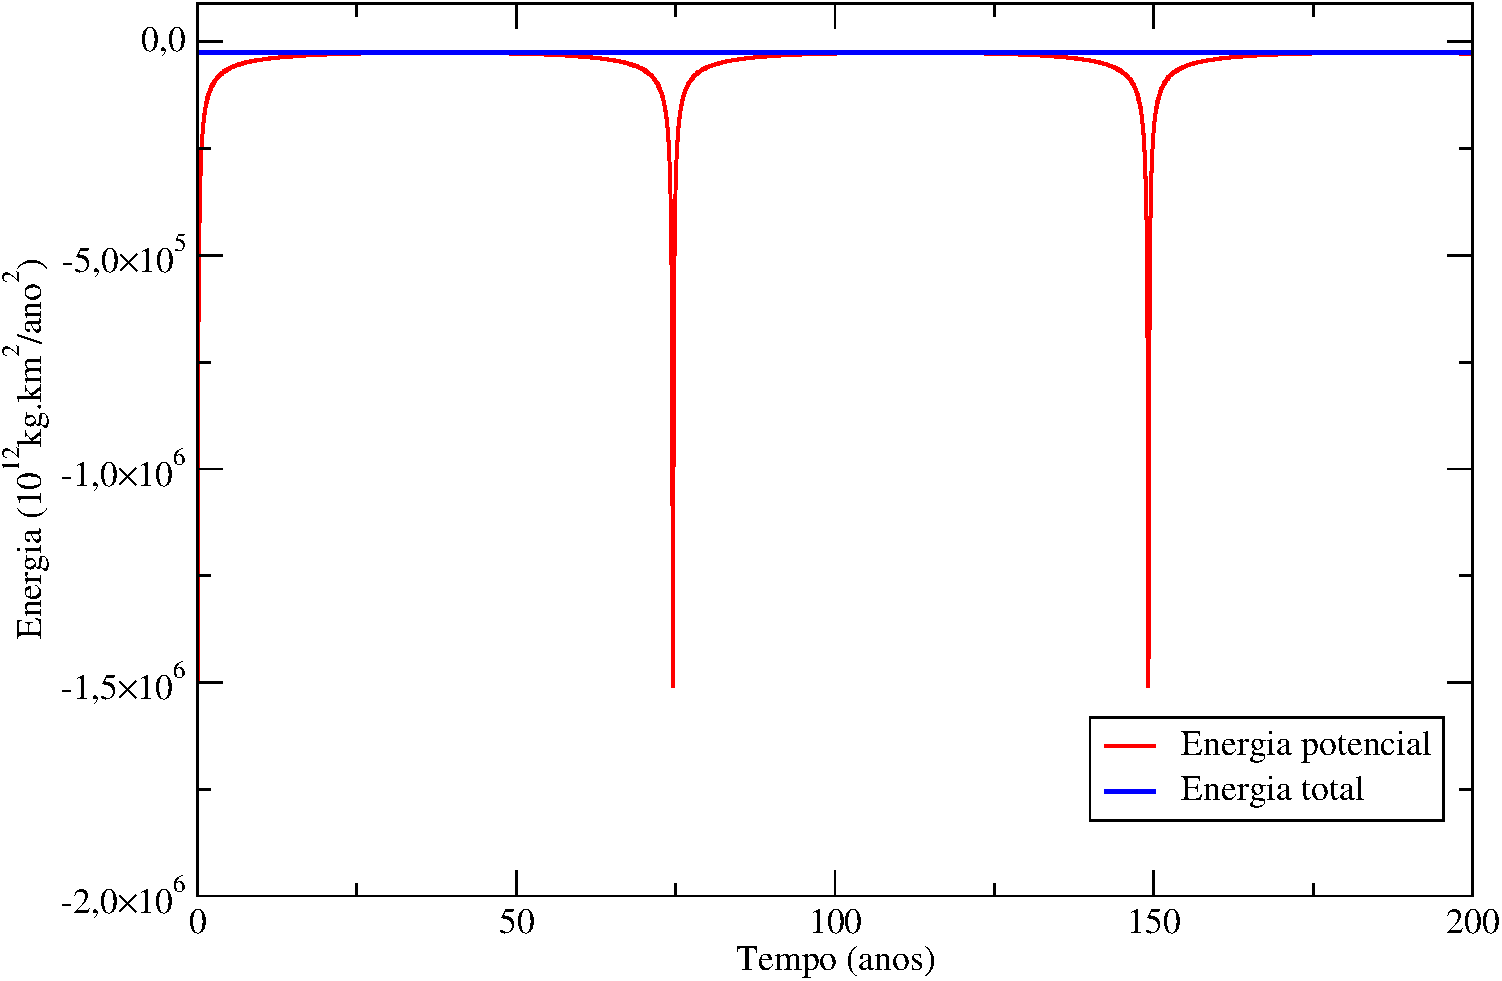
\includegraphics[width=0.447\textwidth]{U.pdf}
\caption{Energia cinética (esquerda) e potencial(direita) em função do tempo.}
\label{3b1}
\end{figure}

Na Figura \ref{3b2} temos o momento angular em função do tempo. À primeira vista, pode parecer que $L$ varia com o tempo, mas deve-se notar que a variação é causada pela precisão numérica do programa. As variações estão somente na nona casa decimal. 

\begin{figure}[!htb]
\centering
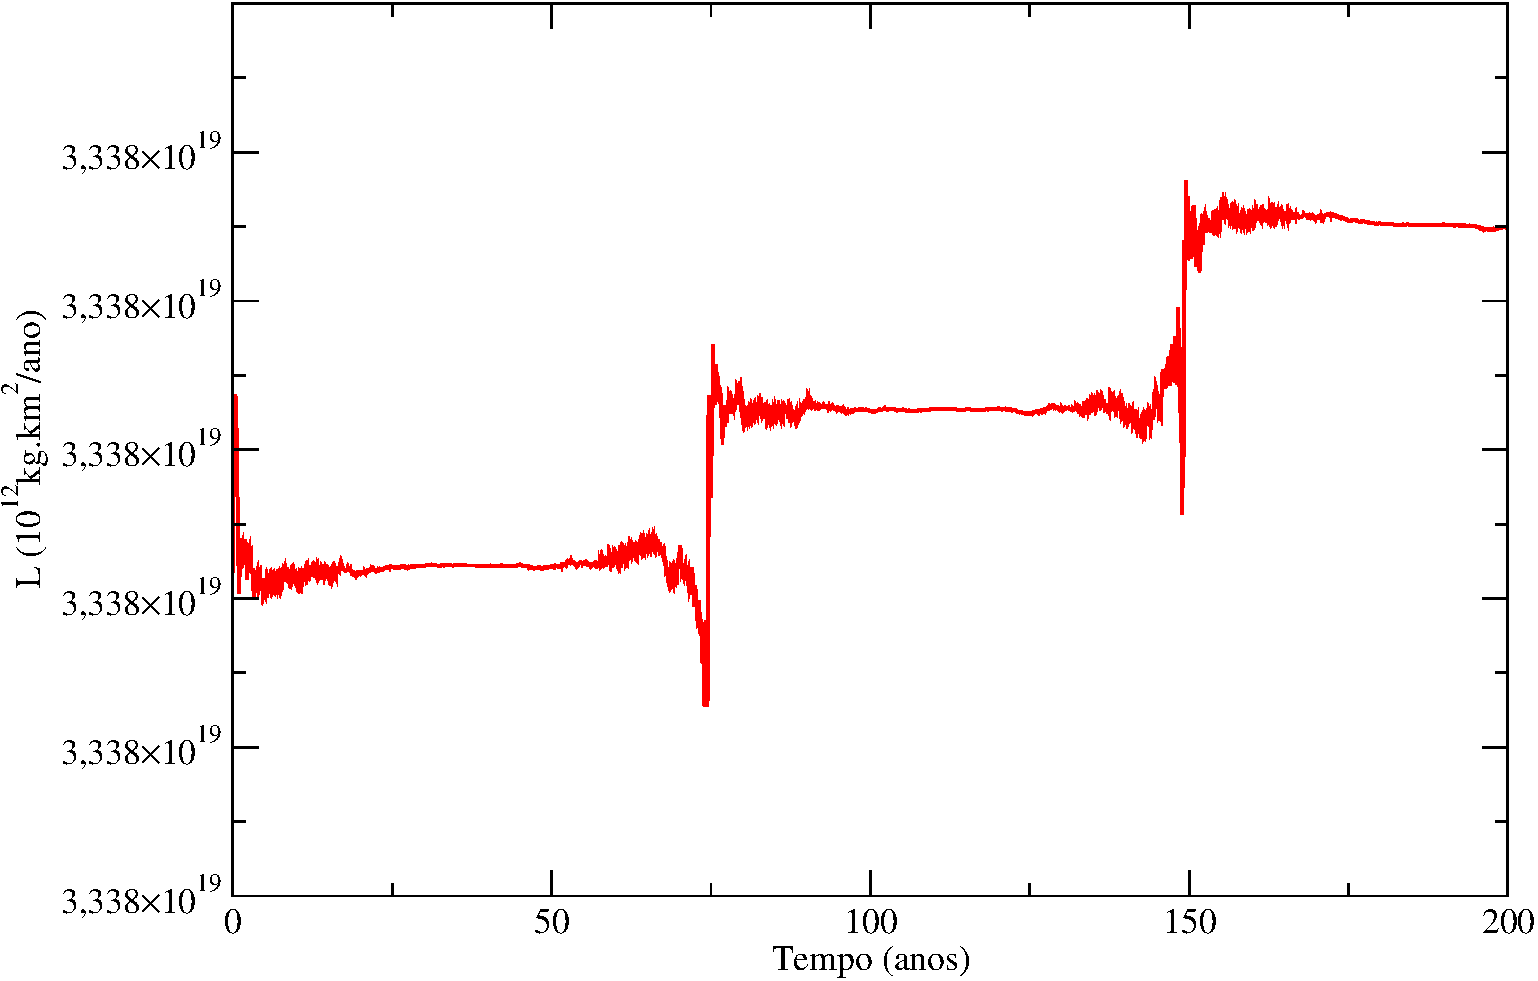
\includegraphics[width=0.447\textwidth]{L2.pdf}
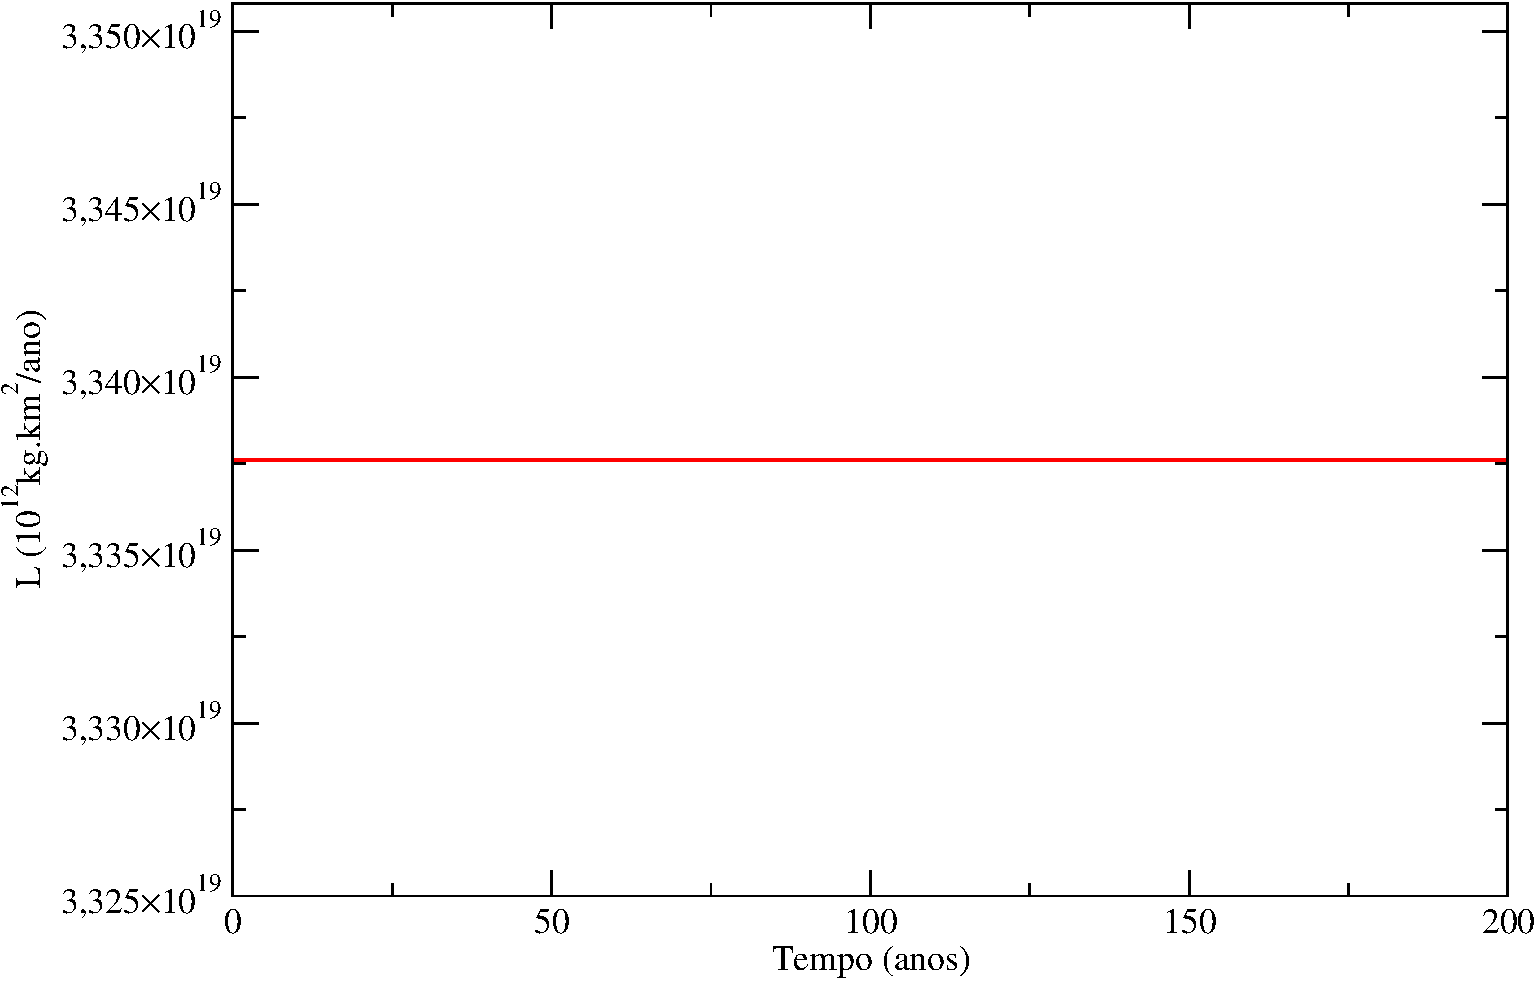
\includegraphics[width=0.447\textwidth]{L.pdf}
\caption{Momento angular em função do tempo. Note que as variações em L são muito menores que 0.1$\%$. }
\label{3b2}
\end{figure}

\subsection*{c)}
Como a energia total (que pode ser visto na Figura \ref{3b1}) é negativa, temos que o sistema forma um estado ligado e as órbitas devem ser fechadas. Utilizando a Figura \ref{3b1} podemos estimar o periodo como sendo $\tau = 74.6$ anos.


\section{Referências}
[1] - Mecânica Analítica - Nivaldo Lemos (Capítulo 7, seção 3.)
\end{document}
